\chapter{CONSTANT pH REPLICA EXCHANGE MOLECULAR DYNAMICS}
\label{ch3}

In this chapter, I will discuss my work with REMD simulations in which the state
parameter---the property exchanged between replicas---is the solution pH.  This
work is reprinted with permission from
\citeauthor*{Swails_JChemTheoryComput_2012_v8_p4393}, \emph{J. Chem. Theory
Comput} \textbf{2012}, \emph{8} 4393--4404. Copyright
\citeyear{Swails_JChemTheoryComput_2012_v8_p4393} American Chemical Society.
\cite{Swails_JChemTheoryComput_2012_v8_p4393}

\section{Constant pH and pK\sub{a} Calculations}

Solution pH is often critical to the proper functioning of biological catalysts.
\cite{Cornish-Bowden1969,White1959} The pH environment of biological systems
influences the ionization equilibria present in the system, thereby affecting
the protonation state of various \emph{titratable residues} in the system. A
titratable residue is any residue that has a pK\sub{a} value within 1 or 2 units
of the biological pH range (which is roughly 1 -- 9). The protonation states of
these residues can have a profound effect on the stability of the system, the
system's interactions with its surroundings, and any catalytic mechanism that
relies on a specific set of protonation states to carry out general acid-base
catalysis or nucleophilic attack. \cite{Tanford_JAmChemSoc_1957_v79_p5333}

Simulations aimed at modeling proteins or nucleic acids must have some method
for assigning protonation states for each titratable residue. Because bond
breaking and bond formation are impossible in classical force fields, each
residue is typically assigned one protonation state and the entire simulation is
run using this set of states. This approach has two drawbacks. First, the
choice of protonation state is often based on the behavior of each titratable
residue when free in solution. This may not be a valid assumption, however,
because the protein or nucleic acid environment can modulate a residue's
protonation state equilibrium. Second, a single protonation state may not
accurately represent the true ensemble of states at the desired pH. If the pH
is close to the pK\sub{a} of a given residue, or if the system populates
conformations in which the dominant protonation state changes, then the true
ensemble is represented by conformations with different protonation states.

The first drawback can be addressed by using tools such as \emph{PROPKA}
\cite{Olsson2011} and \emph{H++}, \cite{Myers_Proteins_2006_v63_p928} which
provide a means to assign protonation states to titratable residues by
calculating the pK\sub{a} of the starting structure. However, this does not
address the possibility that multiple protonation states may be necessary to
build the desired ensemble.

While it may seem that both drawbacks can be addressed by simply running
simulations with every possible set of protonation states, this approach quickly
becomes unwieldy. Given $N$ titratable residues, there are at least $2^N$
distinct protonation states assuming each residue is either protonated or
deprotonated.  With only 10 titratable residues this amounts to a minimum of
1024 distinct simulations!  While most of these states may not be found in the
given ensemble, there is no way to know which ones to exclude \emph{a priori}.
It is important, then, to develop a method capable of directly probing
protonation state equilibria in biological molecules.

In order to probe protonation state equilibria in a thermodynamically meaningful
way, simulations must be run at constant pH. The first approaches for constant
pH simulations used \emph{continuum electrostatics} methods to calculate the
perturbing effect of the system environment on protonation state equilibria
using an implicit solvent model (\eg the Poisson-Boltzmann equation) on a
single structure. \cite{Bashford_Biochemistry_1990_v29_p10219,
Bashford_JMolBiol_1992_v224_p473, Antosiewicz_JMolBiol_1994_v238_p415} These
methods, while sometimes useful for calculating pK\sub{a} values in biological
systems, assume that the full protonation state equilibria can be characterized
with a single structure. In particular, using a single structure neglects the
response of the system relaxing to accommodate the new protonation state. While
the effects of system relaxation has been addressed to some degree by treating
the protein interior with a large dielectric constant,
\cite{Antosiewicz_JMolBiol_1994_v238_p415} this approach assumes an unphysical
homogeneity in the system's dielectric response to protonation state changes.

A more sophisticated approach to incorporating the system response involves
simultaneous sampling of both protonation states and side-chain rotamers.
\cite{Song_JComputChem_2009_v30_p2231} This approach dramatically improves
pK\sub{a} prediction with respect to experiment, but may be insufficient for
systems with large scale conformational changes that cannot be attributed only
to side chain mobility.

To capture the coupled nature of conformational flexibility with protonation
state sampling, several constant pH molecular dynamics (CpHMD) methods have been
proposed. \cite{Baptista_Proteins_1997_v27_p523,
Baptista_JChemPhys_2002_v117_p4184, Burgi_Proteins_2002_v47_p469,
Lee_Proteins_2004_v56_p738, Borjesson_JPhysChemB_2004_v108_p13551,
Mongan_JComputChem_2004_v25_p2038, Khandogin_BiophysJ_2005_v89_p141} These
methods have proven to be powerful tools for pK\sub{a} calculation and
prediction, although there is still room for improvement.
\cite{Alexov_Proteins_2011_v79_p3260} For systems in which some titratable
residues experience large pK\sub{a} shifts, predicted pK\sub{a} values are often
in error by more than 1 pH unit even in the studies that reproduce experimental
values the closest. \cite{Alexov_Proteins_2011_v79_p3260} This is usually a
direct result of insufficient sampling of protonation and conformational states
or a limitation of the underlying model.
\citeauthor{Machuqueiro_Proteins_2011_v79_p3437} have shown that correcting some
of the limitations of the underlying model, such as improving the definition of
the reference compound (whose role is described below in the \emph{Theory}
section) and improving the underlying force field improves results.
\cite{Machuqueiro_Proteins_2011_v79_p3437} Other work has coupled enhanced
sampling techniques, such as accelerated molecular dynamics
\cite{Hamelberg_JChemPhys_2004_v120_p11919}, with CpHMD to show that improved
conformational sampling also improves predicted pK\sub{a}s with respect to
experiment.  \cite{Williams_JChemTheoryComput_2010_v6_p560}
\citeauthor{Webb_Proteins_2011_v79_p685} recently published a systematic study
showing that the errors inherent to experimental measurements are often larger
than those reported, which has important implications for assessing the accuracy
of theoretical predictions. \cite{Webb_Proteins_2011_v79_p685}

\emph{Replica exchange molecular dynamics} (REMD) is a family of extended
ensemble techniques that have been shown to dramatically improve sampling.
\cite{Sugita_ChemPhysLett_1999_v314_p141,
Pitera_ProcNatlAcadSci_2003_v100_p7587, Chodera_JChemPhys_2011_v135_p194110,
Nadler2008, Meng_JChemTheoryComput_2010_v6_p1401,
Meng_JChemTheoryComput_2011_v7_p2721} In REMD simulations, a series of
independent replicas (single MD trajectories of a system) periodically attempt
to exchange information, such as temperature
\cite{Sugita_ChemPhysLett_1999_v314_p141,
Pitera_ProcNatlAcadSci_2003_v100_p7587} and, more recently, pH
\cite{Itoh_Proteins_2011_v79_p3420, Wallace_JChemTheoryComput_2011_v7_p2617} to
sample from an expanded ensemble covering multiple states.

In this study, I implemented the pH-REMD method described by
\citeauthor{Itoh_Proteins_2011_v79_p3420} \cite{Itoh_Proteins_2011_v79_p3420} in
the \emph{sander} module of the Amber \cite{AMBER12} software package. I show
how this method significantly improves sampling compared to CpHMD in hen
egg-white lysozyme (HEWL), a system commonly used as a benchmark for pK\sub{a}
calculations. Titration curves generated using pH-REMD contain significantly
less noise and converge more rapidly than CpHMD, suggesting pH-REMD is a
powerful tool for carrying out pK\sub{a} predictions.

Our group has previously shown that temperature REMD simulations converge
significantly faster with increasing exchange attempt frequency (EAF).
\cite{Sindhikara2008,Sindhikara2010} Here, I show that increasing the EAF in
pH-REMD simulations causes pH-dependent observable properties to converge faster
as well.

In the next sections, I will describe the foundation of the constant pH method
developed by \citeauthor{Mongan_JComputChem_2004_v25_p2038}
\cite{Mongan_JComputChem_2004_v25_p2038} and the corresponding pH-REMD method.
\cite{Itoh_Proteins_2011_v79_p3420, Wallace_JChemTheoryComput_2011_v7_p2617} I
will then describe the details of my study on HEWL followed by the results and
conclusions drawn from that study.

\section{Theory}

Here I will describe the theory behind constant pH simulations, beginning with a
description of the statistical ensemble corresponding to this family of
simulations and following up with an overview of the methods used in this study.

\subsection{The Semi-Grand Ensemble}

At conditions of constant pH, systems no longer obey the constraints of the
typical canonical ensemble presented in the opening chapter. Instead, the
chemical potential of hydronium---related directly to the solution pH by Eq.
\ref{eq3:ChemicalPotential}---is held constant, thereby allowing the H\super{+}
count to fluctuate.

\begin{align}
   \mu ^ {H^+} & = \frac {\partial G} {\partial N^{H^+}} \nonumber \\
               & = -kT\ln [H^+] \nonumber \\
               & = -kT\ln (10) \log [H^+] \nonumber \\
               & = kT\ln (10)\, pH
   \label{eq3:ChemicalPotential}
\end{align}
where $\mu_{H^+}$ is the chemical potential of hydronium and the activity of the
hydronium ion has been replaced by the concentration due to the very low
concentrations in which it is typically present in biological systems. Looking
back at Eq. \ref{eq1:GrandCanonicalPF}, we can calculate the partition function
of the semi-grand canonical ensemble using Eq. \ref{eq3:SemiGrandPF},
introducing a pH-dependence in our sampling scheme.

\begin{align}
   \Xi(\mu ^ {H^+}, V, T) & = \sum _ {N^{H^+}} Q(N, V, T) \exp(\beta RT N^{H^+}
                  \ln(10)\, pH) \nonumber \\
                          & = \sum _ {N^{H^+}} Q(N, V, T) \exp(N^{H^+} \ln(10)\,
                  pH)
   \label{eq3:SemiGrandPF}
\end{align}

\subsection{CpHMD}

I used the constant pH molecular dynamics (CpHMD) method developed by
\citeauthor{Mongan_JComputChem_2004_v25_p2038}
\cite{Mongan_JComputChem_2004_v25_p2038} that employs Monte Carlo transitions
between discrete protonation states at periodic intervals during a MD simulation
to probe protonation state equilibria. In this CpHMD implementation, both the
dynamics and the MC protonation state sampling are performed in Generalized Born
implicit solvent. After a predetermined number of steps, the MD is halted and a
protonation state change is attempted by evaluating the energetic cost of that
proposed change, calculated according to Eq. \ref{eq3:ProtChange}.
\cite{Mongan_JComputChem_2004_v25_p2038}
\begin{equation}
   \Delta G = k _ B T \left( pH - pK _ {a,ref} \right) \ln 10 + \Delta G _
         {elec} - \Delta G _ {elec,ref}
   \label{eq3:ProtChange}
\end{equation}
Eq. \ref{eq3:ProtChange} represents a free energy change of protonating or
deprotonating a titratable residue embedded in a biological system with respect
to a predefined reference compound. The reference compound is a monomer of the
titratable residue capped with small, neutral functional groups. In Eq.
\ref{eq3:ProtChange}, $\Delta G _ {elec}$ is calculated by taking the difference
of the electrostatic energy between the proposed and existing protonation
states. \cite{Mongan_JComputChem_2004_v25_p2038}

Directly calculating the free energy change associated with protonation or
deprotonation is difficult because evaluating the energetic cost of desolvating
a free proton and making and breaking chemical bonds is impossible in a
classical mechanical framework. Therefore, we calculate the free energy cost of
this protonation state change by comparing the free energy of the protonation
state change to $\Delta G _ {elec,ref}$ in Eq. \ref{eq3:ProtChange}, a
precomputed free energy for the reference compound that is adjusted to reproduce
experimental pK\sub{a} values. Eq. \ref{eq3:ProtChange}, then, represents a
shift in the pK\sub{a} of a titratable residue in a biological system from its
value free in solution. The reference compound pK\sub{a} values used in the
Amber CpHMD implementation \cite{Mongan_JComputChem_2004_v25_p2038} are shown in
Table
\ref{tbl3:refpkas}.

\begin{table}
  \caption{Reference pK\sub{a} values for the acidic residues treated in this
           study. Values are the same as those used in the original Amber CpHMD
           implementation.\cite{Mongan_JComputChem_2004_v25_p2038}}
  \label{tbl3:refpkas}
  \begin{tabular}{lc}
    \hline
    Residue & Reference pK\sub{a} \\
    \hline
    Aspartate & 4.0 \\
    Glutamate & 4.4 \\
    Histidine (H$^\delta$) & 7.1 \\
    Histidine (H$^\epsilon$) & 6.5 \\
    \hline
  \end{tabular}
\end{table}

Running a CpHMD simulation, we obtain an ensemble consisting of multiple
protonation states properly weighted for the semi-grand canonical ensemble, the
thermodynamic ensemble corresponding to constant temperature, volume (or
pressure) and chemical potential of hydronium (\ie constant pH).
\cite{Baptista_JChemPhys_2002_v117_p4184} Because the simulation is assumed to
be ergodic, the deprotonation fraction can be calculated by simply counting the
fraction of ensemble members in which the residue is deprotonated. Multiple
CpHMD simulations must be run with a range of pHs to calculate pK\sub{a} values
for titratable residues in biological systems by fitting a titration curve to
the data.

Running a simulation with an expanded ensemble so each CpHMD simulation is in
equilibrium with simulations at different pHs can further enhance sampling from
the desired semi-grand canonical ensemble. For this, we turn to the pH-REMD
method.

\subsection{pH-REMD}

Replica exchange simulations at constant pH (pH-REMD) is a variant of replica
exchange in which each replica is simulated at a separate pH. The full pH-REMD
simulation represents an expanded ensemble in which each replica samples
conformations with a fixed pH and samples different pH values at a fixed
conformation.

In this study, I implemented the pH-REMD method introduced by
\citeauthor{Itoh_Proteins_2011_v79_p3420} \cite{Itoh_Proteins_2011_v79_p3420} in
the \emph{sander} module of Amber.  \cite{AMBER12} In pH-REMD, adjacent replicas
in the pH ladder swap pH with the Monte Carlo exchange probability
\begin{equation}
   P _ {i \rightarrow j} = \min \left \lbrace 1, \exp \left[ \ln 10 \left( N _ i
            - N _ j \right) \left( pH_i - pH_j \right) \right] \right \rbrace
   \label{eq3:ExchSucc}
\end{equation}
for replicas $i$ and $j$ where $N_i$ is the number of titratable protons present
in replica \emph{i} and $pH_i$ is the pH of replica $i$ prior to the exchange
attempt.

Our group recently developed a different pH-REMD method in which replica
exchanges are attempted via Hamiltonian exchange where only atomic coordinates
are swapped. \cite{Dashti_JPhysChemB_2012_v116_p8805} In contrast, the currently
proposed method only swaps the solution pH between replicas. For large systems
with more than 3 -- 5 titratable residues, the proposed method of swapping
solution pH between replicas achieves more efficient replica exchanges than the
variant employing Hamiltonian exchange. For HEWL, specifically, the Hamiltonian
REMD variant experienced an exchange success rate of $<0.01\%$, which is
effectively indistinguishable from CpHMD simulations.

\section{Methods}

\subsection{Starting Structure}

I chose to study hen egg white lysozyme because it is well-characterized both
experimentally \cite{Takahashi_Biopolymers_1992_v32_p897,
Bartik_BiophysJ_1994_v66_p1180, Webb_Proteins_2011_v79_p685} and
computationally. \cite{Mongan_JComputChem_2004_v25_p2038,
Demchuk_JPhysChem_1996_v100_p17373, Wallace_JChemTheoryComput_2011_v7_p2617} I
chose the structure from the protein data bank (PDB) with the code 1AKI
\cite{Artymiuk_ActaCrystB_1982_v38_p778} because it was the focus of Mongan's
original study. \cite{Mongan_JComputChem_2004_v25_p2038}

The topology file was prepared in the \emph{tleap} module of AmberTools 12 using
the Amber \emph{ff10} force field, which is equivalent to \emph{ff99SB}
\cite{Hornak_Proteins_2006_v65_p712} for proteins. Crystallographic water
molecules were removed from the starting structures, and \emph{tleap} added all
hydrogen atoms.  Finally, the \emph{mbondi2} intrinsic radii for implicit
solvent calculations were selected in \emph{tleap} to be consistent with the
initial implementation of CpHMD. \cite{Mongan_JComputChem_2004_v25_p2038}

\subsection{Molecular Dynamics}

To be consistent with the original implementation, the Generalized Born model
described by \citeauthor{Onufriev_Proteins_2004_v55_p383}
\cite{Onufriev_Proteins_2004_v55_p383} (corresponding to the input parameter
\emph{igb=2} for Amber programs) was used with the salt concentration, modeled
as a Debye screening parameter, set to 0.1 M in every simulation.
\cite{Mongan_JComputChem_2004_v25_p2038} Due to the long-range nature of the
electrostatic forces, I always used an infinite cutoff for non-bonded
interactions.

Each starting structure was minimized using 50 steps of steepest descent
followed by 950 steps of conjugate gradient with 10 kcal mol\super{-1}
\AA\super{-2} restraints on the backbone atoms to relieve bad contacts. Then,
the minimized structure was heated by varying the target temperature linearly
from 10 K to 300 K for 667 ps, keeping weak restraints---1 kcal mol\super{-1}
\AA\super{-2}--on the backbone. I used the Langevin thermostat with a
collision frequency of 5 ps\super{-1} to control the temperature. These
simulations were performed using the \emph{pmemd} module of the Amber 12 program
suite. \cite{AMBER12}

After heating, each structure was further run at 300 K for 1 ns with 0.1 kcal
mol\super{-1} \AA\super{-2} restraints on the backbone. Each titratable
carboxylate was deprotonated and the histidine was protonated, and no
protonation state changes were attempted during the simulation. Next, the
resulting structure was used to start 16 ns of CpHMD at pH values spanning 2 to
7 with an interval of 0.5. Only the 10 acidic residues---the aspartates,
glutamates, and histidines---were titrated because HEWL is catalytically active
at low pH \cite{Vocadlo_Nature_2001_v412_p835} and 1AKI was solved in these
conditions. I used a 2 fs time step and attempted protonation state changes
every 5 steps. The Langevin thermostat with a collision frequency of 10
ps\super{-1} was used to control the temperature, and simulations were begun
with a different random seed to avoid synchronization artifacts.
\cite{Sindhikara_JChemTheoryComput_2009_v5_p1624} I used the \emph{sander}
module of Amber 12 for each of these simulations.

\subsection{Replica Exchange}

All pH-REMD simulations were run with 12 equally spaced replicas at pH values
spanning 2 to 7.5---identical to the pH values used for the CpHMD simulations
with the addition of a replica at pH 7.5. The additional replica is necessary
because the REMD implementation in \emph{sander} requires an even number of
replicas so that each replica has a partner for each exchange attempt. The
structures obtained after 1 ns of CpHMD simulation for each pH were used as the
starting structure for the replica exchange simulations (the structure from
CpHMD run at pH 7 was used for the replica run at pH 7.5 as well).

I ran pH-REMD simulations with exchange attempt frequencies (EAFs) (\ie the
frequency with which replicas attempt to swap pH values) equal to 50
ps\super{-1}, 10 ps\super{-1}, 5 ps\super{-1}, and 0.5 ps\super{-1} to assess
the effect of EAF on the convergence of observable properties. This corresponds
to attempting exchanges every 10, 50, 100, and 1000 steps, respectively. All
pH-REMD simulations were run for 15 ns. I note here that the CpHMD simulations
are equivalent to a REMD simulation with an EAF equal to 0.

I used an in-house, modified version of \emph{sander} in which I implemented
pH-REMD for these simulations and wrote in-house scripts to extract pH-based
titration data from the ensemble of replica-based files. The replica at pH 7.5
was ignored in all pH-REMD analyses so the simulations could be compared fairly.

\section{Results and Discussion}

CpHMD methods must sample both protonation states and conformation states to
build a thermodynamically meaningful ensemble. Here I will discuss how well
CpHMD, as implemented in Amber, \cite{Mongan_JComputChem_2004_v25_p2038} samples
from the desired ensemble. I then analyze how pH-REMD affects protonation and
conformational state sampling compared to CpHMD, and how effective these tools
are for pK\sub{a} prediction.

\subsection{Simulation Stability}
CpHMD involves instantaneous changes in the charge distribution of the protein
as the protonation states are changed. Therefore, it is important to verify
that trajectories generated from CpHMD and pH-REMD remain stable with respect to
secondary and tertiary structure during the course of the simulation.

\citeauthor{Mongan_JComputChem_2004_v25_p2038}
\cite{Mongan_JComputChem_2004_v25_p2038} showed that temperature and energy
fluctuations greater than those obtained with standard MD (\ie MD simulations
with static protonation states) were minimal during the course of a 1 ns
simulation. Most of the energy fluctuations arise from the intrinsic response of
the force field to the new charge state.

To analyze structural stability, I plotted the root mean squared deviation
(RMSD) of every $\alpha$-carbon in the protein with respect to the minimized
crystal structure vs. time. The results from CpHMD and pH-REMD simulations are
shown in Fig. \ref{fig3:RMSD} for the lowest pH, 2; the highest pH, 7; and an
intermediate pH, 4.5. The RMSDs are bounded below 4 \AA, suggesting that the
trajectories remain stable for both CpHMD and pH-REMD during the entire
simulation.

\begin{figure}
 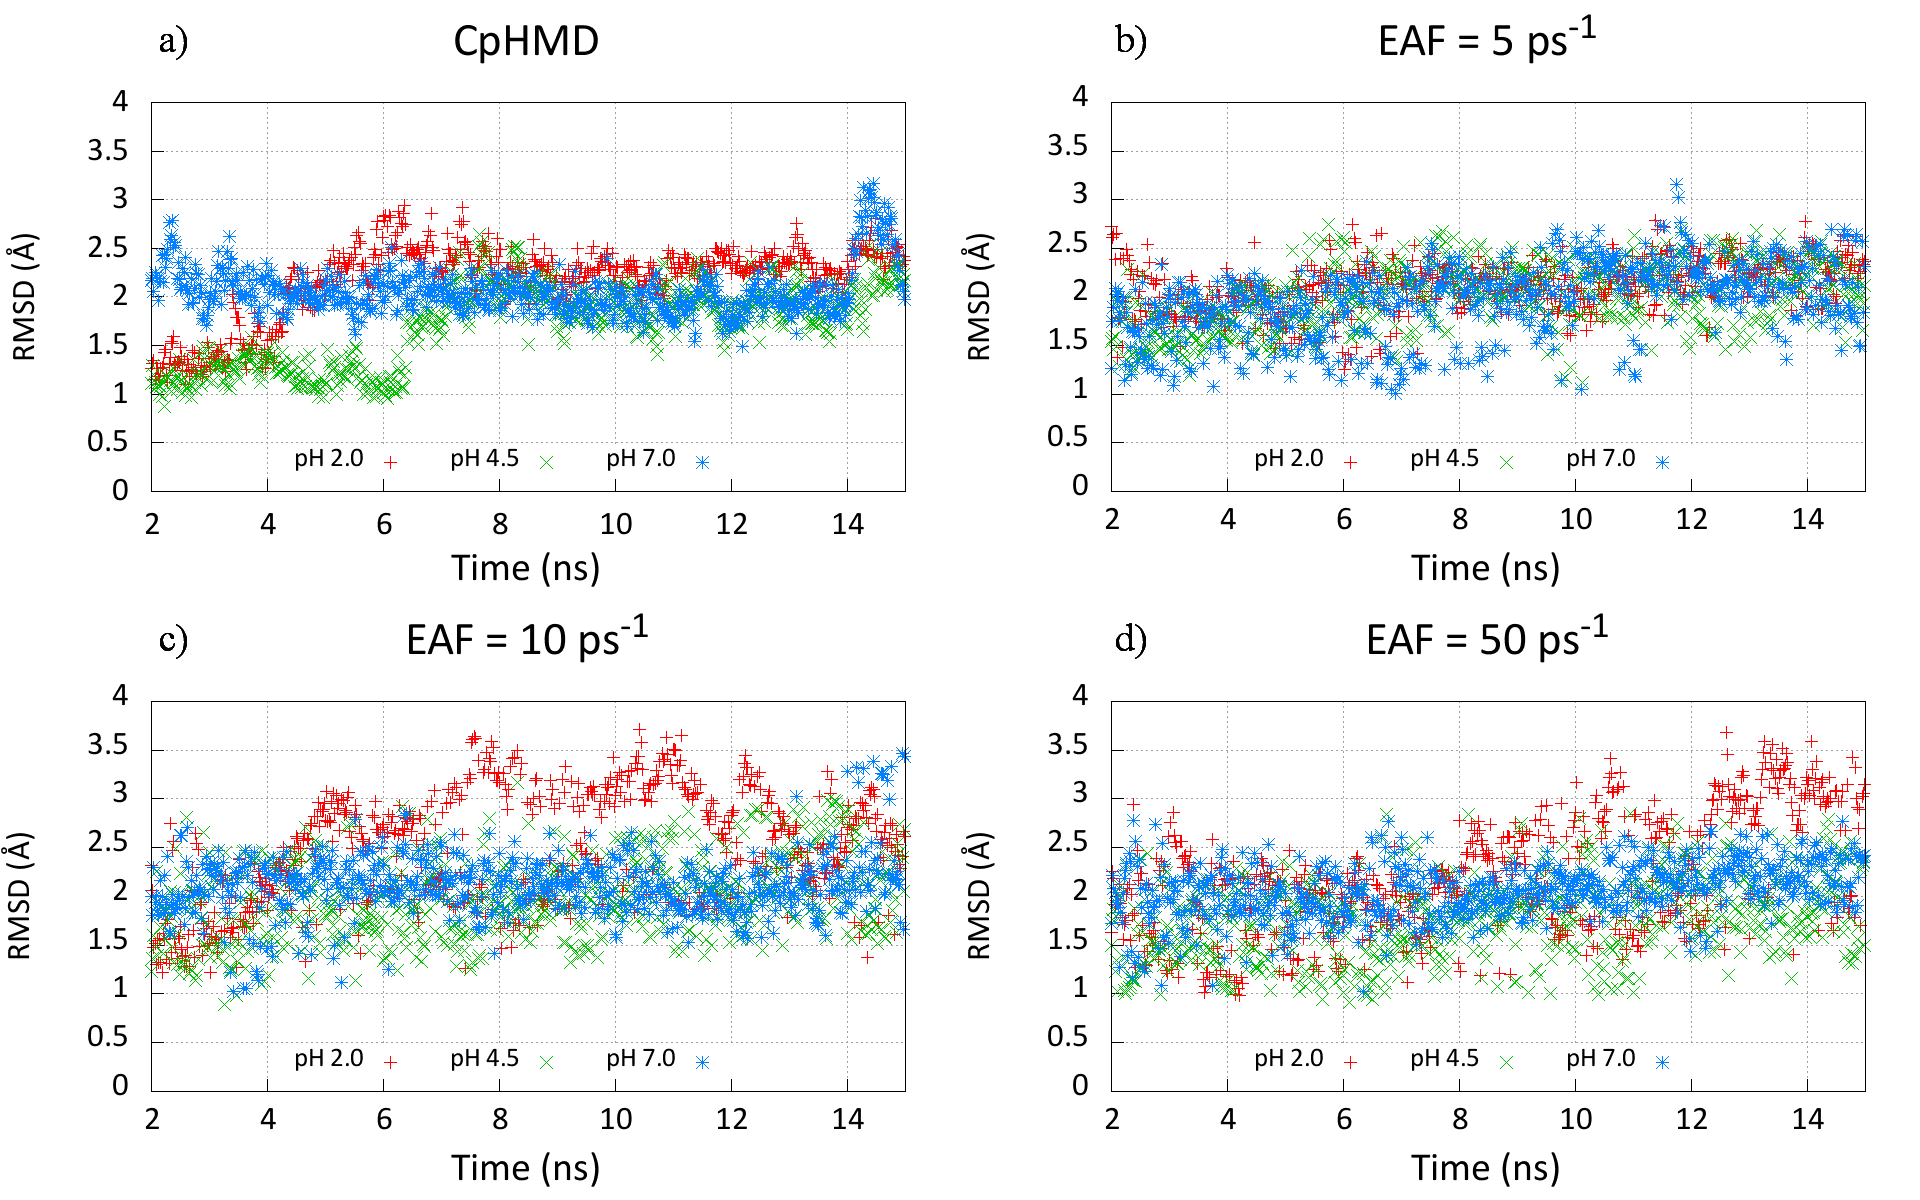
\includegraphics[width=6.5in, height=4.06in]{1AKI_RMSD_Comparison.png}
 \caption[RMSD plots for CpHMD simulations (a) and pH-REMD simulations at
          different exchange attempt frequencies (b-d) as a function of time]
         {RMSD plots for CpHMD simulations (a) and pH-REMD simulations at
          different exchange attempt frequencies (b-d) as a function of time
          throughout the simulation. The first nanosecond is excluded, as
          described in \emph{Methods}. The RMSD is plotted with respect to the
          minimized crystal structure 1AKI and are shown for one low, one
          medium, and one high pH simulation (2, 4.5, and 7, respectively).}
 \label{fig3:RMSD}
\end{figure}

\subsection{Accuracy of Predicted pK\sub{a}s}

One of the goals of any constant pH simulation method is to accurately predict
pK\sub{a} values of titratable residues. The pK\sub{a} of each residue was
calculated by using the \emph{Levenberg-Marquardt} non-linear optimization
method to fit the titration data at each pH to the standard Hill equation shown
below:
\begin{equation}
 f_{d} = \frac 1 {10 ^ {n \left( pK_a - pH \right)} + 1}
 \label{eq3:hill}
\end{equation}
where $f_d$ is the fraction of the total simulation that the titratable residue
spent in a deprotonated state.

\begin{table}
  \caption[pK\sub{a} and Hill coefficients for each residue taken from each set
           of simulations. The pK\sub{a}s and Hill coefficients (\textit{n})
           are shown for each EAF.]
          {pK\sub{a} and Hill coefficients for each residue taken from each set
           of simulations. The pK\sub{a}s and Hill coefficients (\textit{n})
           are shown for each EAF. pK\sub{a} root mean square errors (RMSEs)
           from the \super{13}C-NMR experimental values published by
           \citeauthor{Webb_Proteins_2011_v79_p685}
           \cite{Webb_Proteins_2011_v79_p685} are shown in the last row.
           Asp 66 was problematic because it is positioned between several
           Arginine residues, causing it to resist protonation. When it
           significantly impacts the RMSE, the RMSE for all residues
           \emph{except} Asp 66 is shown in parentheses next to the total RMSE.}
  \label{tbl3:pkas}
  \begin{tabular}{lrcrcccc}
    \hline
    & \multicolumn{2}{c}{CpHMD} & \multicolumn{2}{c}{EAF=0.5 ps\super{-1}} & 
      \multicolumn{2}{c}{EAF=50.0 ps\super{-1}} & \\
    Residue & pK\sub{a} & \textit{n} & pK\sub{a} & \textit{n} &  
    pK\sub{a} & \textit{n} & Expt. pK\sub{a} \\
    \hline
    GLU 7 & 3.62 & 1.16 & 3.60 & 0.88 &  3.84 & 0.96 & 2.6 $\pm$ 0.2 \\
    HIS 15 & 5.96 & 1.05 & 5.74 & 1.09 &  5.90 & 0.97 & 5.5 $\pm$ 0.2 \\
    ASP 18 & 2.26 & 1.11 & 2.01 & 0.94 &  2.01 & 0.89 & 2.8 $\pm$ 0.3 \\
    GLU 35 & 5.67 & 3.82 & 5.44 & 1.16 &  4.98 & 0.98 & 6.1 $\pm$ 0.4 \\
    ASP 48 & 1.22 & 0.43 & 1.11 & 0.71 &  1.99 & 0.83 & 1.4 $\pm$ 0.2 \\
    ASP 52 & 2.69 & 1.16 & 2.37 & 0.96 &  2.30 & 0.75 & 3.6 $\pm$ 0.3 \\
    ASP 66 & -18.13 & 0.11 & -3.17 & 0.49 & 1.53 & 1.19 & 1.2 $\pm$ 0.2 \\
    ASP 87 & 2.52 & 0.81 & 2.61 & 0.81 & 2.66 & 0.91 & 2.2 $\pm$ 0.1 \\
    ASP 101 & 3.69 & 2.10 & 3.66 & 1.00 & 3.57 & 0.87 & 4.5 $\pm$ 0.1 \\
    ASP 119 & 2.26 & 0.98 & 2.73 & 1.04 & 2.43 & 0.96 & 3.5 $\pm$ 0.3 \\
    \\
    RMSE & \multicolumn{2}{c}{6.15 (0.74)} & 
                \multicolumn{2}{c}{1.56 (0.76)} & 
                \multicolumn{2}{c}{0.89} &
                --- \\
    \hline
  \end{tabular}
\end{table}

Table \ref{tbl3:pkas} shows the calculated pK\sub{a} values for each titratable
residue calculated from Eq. \ref{eq3:hill} for select exchange attempt
frequencies.  Hill coefficients that differ significantly from 1 imply either
that the pK\sub{a} of that residue displays significant
non-Henderson-Hasselbalch (non-HH) behavior, or that protonation space is poorly
sampled at some pH values, depending on how well Eq. \ref{eq3:hill} fits the
data. If Eq. \ref{eq3:hill} fits the data poorly, then poor protonation state
sampling is at least partially responsible for the deviation of the Hill
coefficient from 1. Because only the CpHMD simulations show several residues
whose Hill coefficient deviates substantially from 1, we conclude that pH-REMD
improves sampling from the desired ensemble.

\subsection{Enhancing Protonation State Sampling with pH-REMD}

Replica exchange methodologies are well-known to improve sampling in the desired
ensemble \cite{Sugita_ChemPhysLett_1999_v314_p141,
Chodera_JChemPhys_2011_v135_p194110} as long as replicas traverse the
state-space ladder regularly.  If replica exchange attempts always fail, the
simulation does not benefit from those attempts.  In our pH-REMD simulations,
exchange attempts between replicas with neighboring pH values (\ie replicas with
solution pHs separated by 0.5 pH units) succeeded between 40\% to 98\% of the
time, displaying very efficient traversal of the pH-space replica ladder. Here I
will discuss the extent to which pH-REMD, with different exchange attempt
frequencies (EAFs), improves protonation state sampling compared to CpHMD.

\begin{figure}
 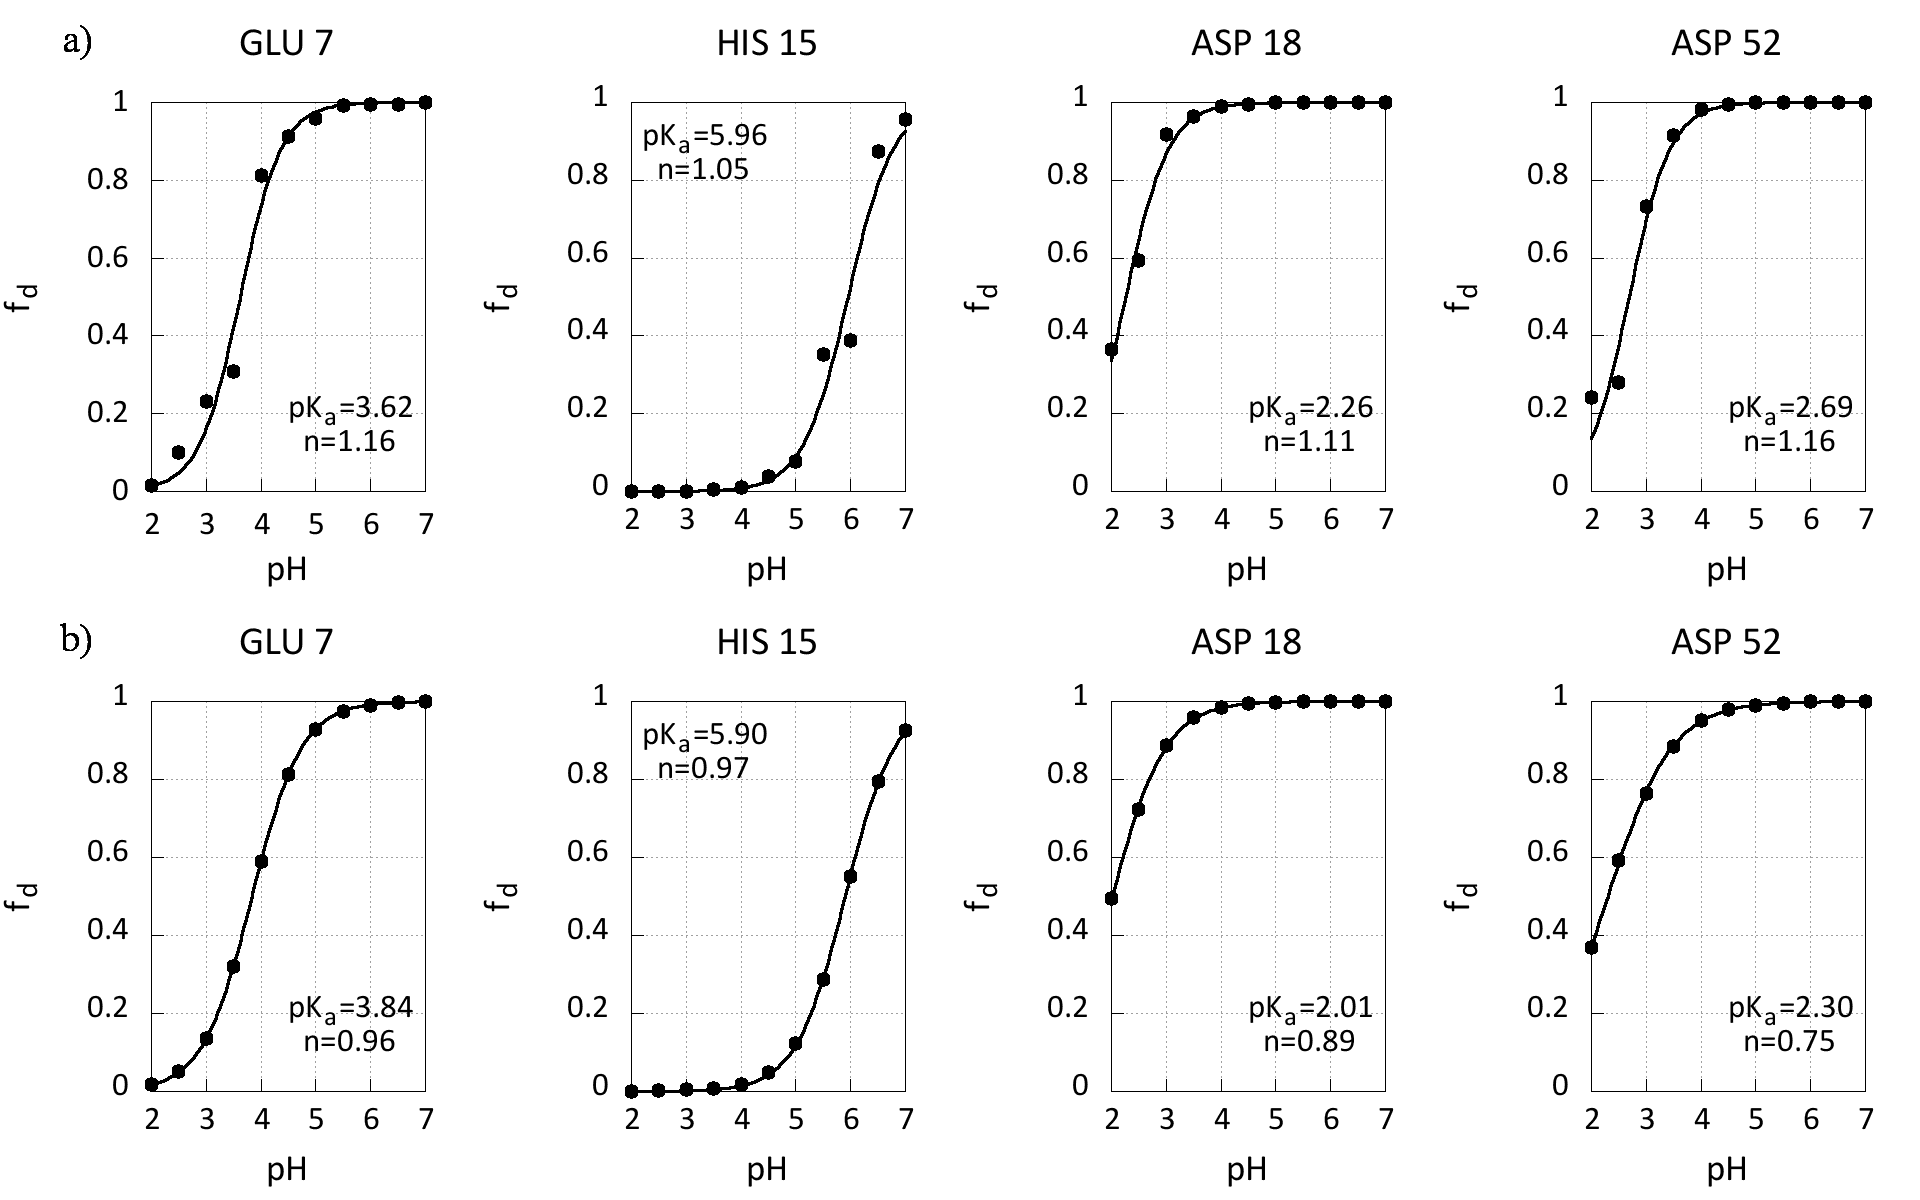
\includegraphics[width=6.5in, height=4.06in]{Comparison_good_curves.png}
 \caption{Titration curves obtained with (a) EAF=0 ps\super{-1}, and (b) EAF=50
          ps\super{-1}. The data for these residues show the best fit to Eq.
          \ref{eq3:hill} for the CpHMD simulations.}
 \label{fig3:GoodTitr}
\end{figure}

I show sample titration curves for simulations with no exchange attempts and
simulations in which replica exchanges were attempted with a frequency of 50
ps\super{-1}.  Residues for which `good' titration curves are obtained with
CpHMD are shown in Fig. \ref{fig3:GoodTitr}.  I characterize `good` titration
curves by small deviations of each point from the fitted titration curve and
Hill coefficients between 0.5 and 1.5. Residues that show poor titration curves
for CpHMD---characterized by large deviations of points from the fitted
titration curve and/or Hill coefficients significantly shifted from 1---are
shown in Fig. \ref{fig3:BadTitr}.

\begin{figure}
 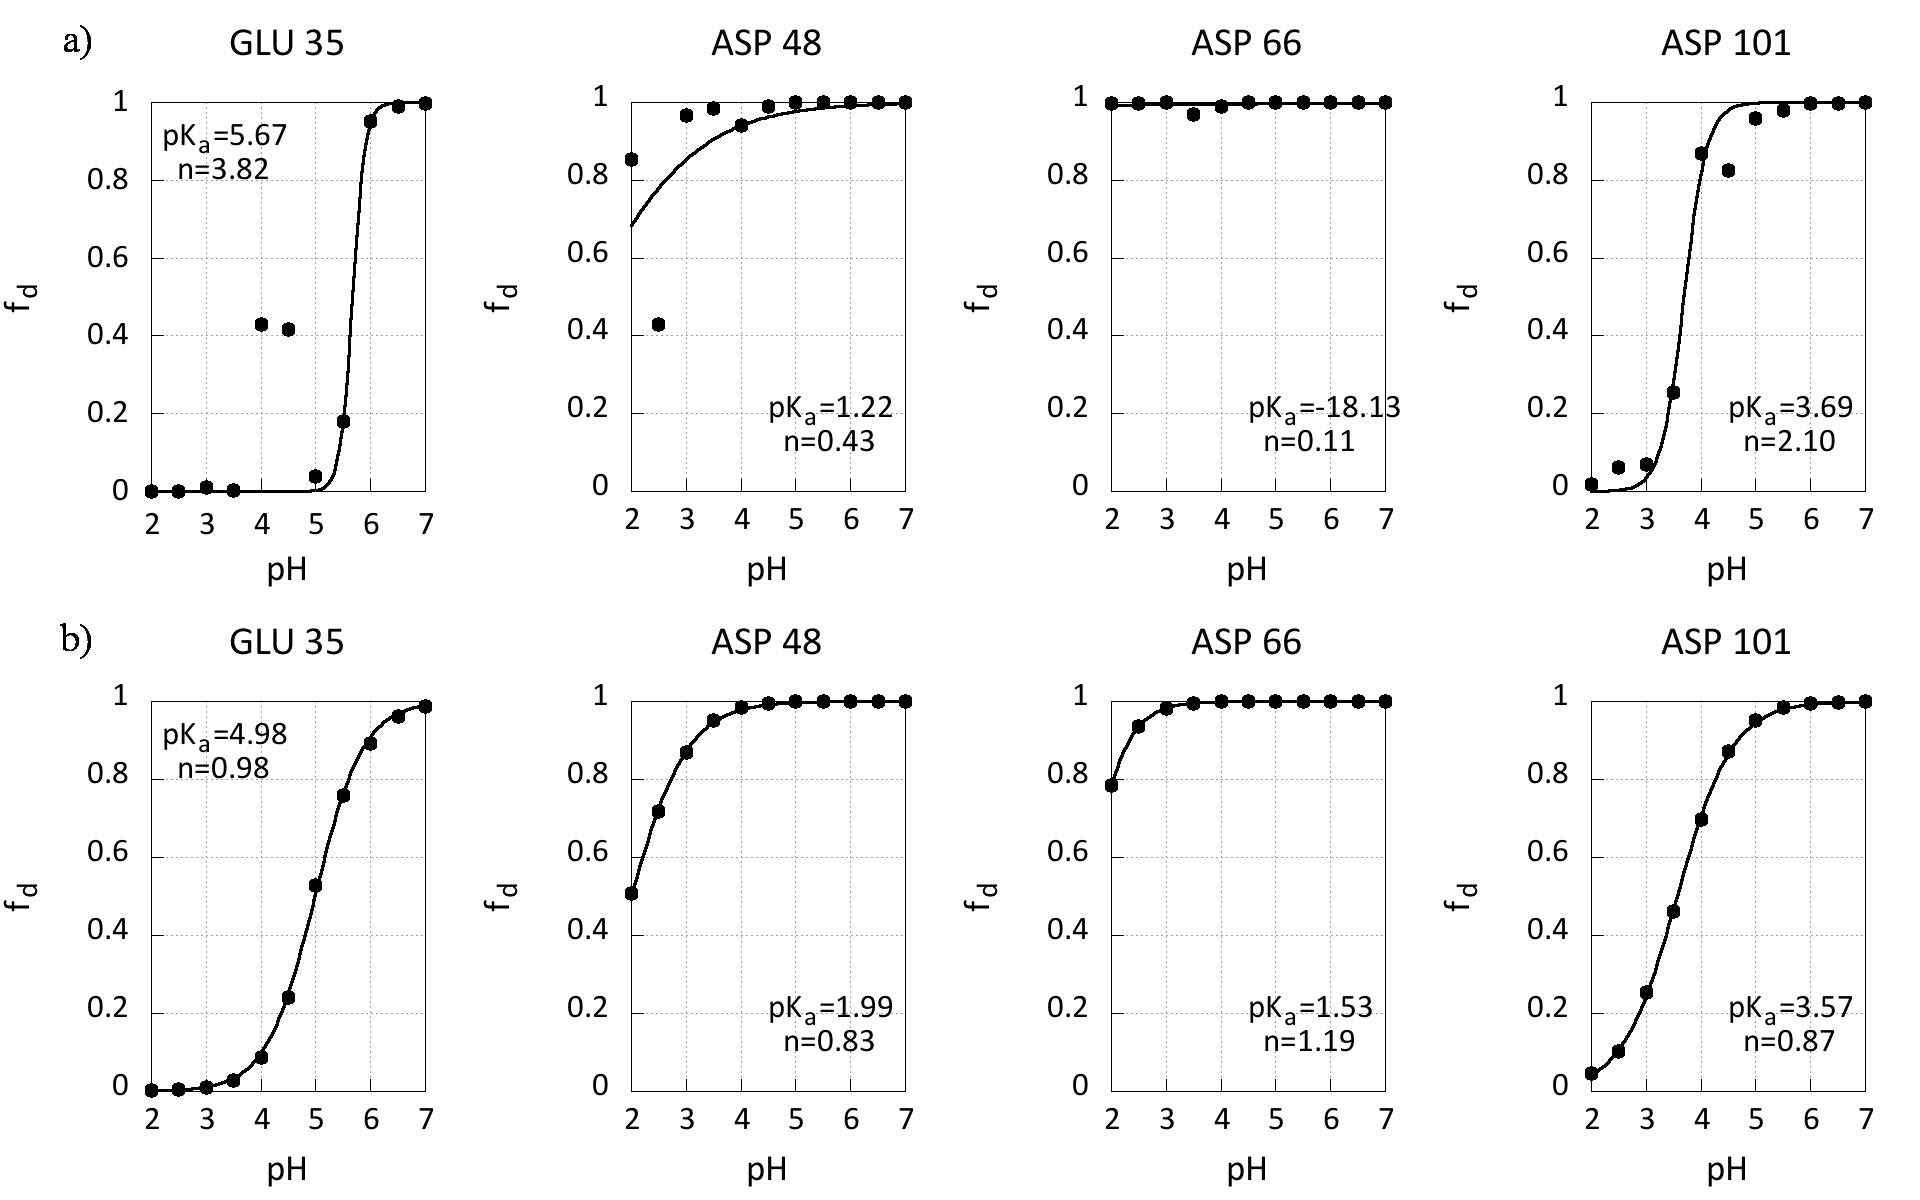
\includegraphics[width=6.5in, height=4.06in]{Comparison_bad_curves.png}
 \caption{Titration curves obtained with (a) EAF=0 ps\super{-1} and (b) EAF=50
          ps\super{-1}. The data for these residues have the poorest fit to Eq.
          \ref{eq3:hill} for the CpHMD simulations.}
 \label{fig3:BadTitr}
\end{figure}

Figure \ref{fig3:GoodTitr} shows that even when CpHMD generates data that
closely fit Eq.  \ref{eq3:hill}, using pH-REMD still improves the fit. More
drastic improvement is shown in Fig. \ref{fig3:BadTitr} where CpHMD performs
poorly because some residues become conformationally trapped at several pHs,
impacting protonation state sampling and skewing the points away from the
titration curve.

The quality of the fits can be quantified by measuring the deviation of each
point from the fitted equation according to Eq. \ref{eq3:fit_quality}
\begin{equation}
 RSS = \sum_{points} \left( O(x) - E(x) \right) ^ 2
 \label{eq3:fit_quality}
\end{equation}
where $RSS$ is the residual sum of squares, $O(x)$ is the actual data point, and
$E(x)$ is the value of the fitted equation at that value of $x$. Eq.
\ref{eq3:fit_quality} provides an easy way to quantitatively evaluate how well
the titration data from the pH-REMD simulations fit Eq. \ref{eq3:hill} compared
to the CpHMD simulations.  The results for the 8 residues plotted in Figs.
\ref{fig3:GoodTitr} and \ref{fig3:BadTitr} are shown in Table \ref{tbl3:fits}.

\begin{table}
 \caption[Value of $RSS$ according to Eq. \ref{eq3:fit_quality} for the 8
          residues shown in Figs. \ref{fig3:GoodTitr} and \ref{fig3:BadTitr}.
          Larger values represent more deviation from the fitted curve]
         {Value of $RSS$ according to Eq. \ref{eq3:fit_quality} for the 8
          residues shown in Figs. \ref{fig3:GoodTitr} and \ref{fig3:BadTitr}.
          Larger values represent more deviation from the fitted curve, whereas
          a value of 0 represents a perfect fit. The `good' titratable residues
          (Fig.  \ref{fig3:GoodTitr}) are the first 4 entries and the `bad'
          titratable residues (Fig. \ref{fig3:BadTitr}) are the last 4 entries.}
 \label{tbl3:fits}
 \begin{tabular}{ccc}
  \hline
  Residue & $RSS$ (CpHMD) & $RSS$ (EAF=50 ps\super{-1}) \\
  \hline
  GLU 7 & $2.7 \times 10 ^ {-2}$ & $7.9 \times 10 ^ {-5}$ \\
  HIS 15 & $3.8 \times 10 ^ {-2}$ & $2.7 \times 10 ^ {-5}$ \\
  ASP 18 & $6.3 \times 10 ^ {-3}$ & $3.3 \times 10 ^ {-5}$ \\
  ASP 52 & $2.2 \times 10 ^ {-2}$ & $1.3 \times 10 ^ {-3}$ \\
  GLU 35 & $3.6 \times 10 ^ {-1}$ & $4.2 \times 10 ^ {-4}$ \\
  ASP 48 & $1.7 \times 10 ^ {-1}$ & $2.4 \times 10 ^ {-5}$ \\
  ASP 66 & $8.2 \times 10 ^ {-4}$ & $2.9 \times 10 ^ {-4}$ \\
  ASP 101 & $3.4 \times 10 ^ {-2}$ & $2.7 \times 10 ^ {-4}$ \\
  \hline
 \end{tabular}
\end{table}

The improvement by using pH-REMD over conventional CpHMD, already apparent by
viewing Figs. \ref{fig3:GoodTitr} and \ref{fig3:BadTitr}, is striking as measured in
Table \ref{tbl3:fits}.  Even when CpHMD performs well, pH-REMD results in an
improvement of 2 -- 3 orders of magnitude in the $RSS$ metric, and results in at
least another order of magnitude of improvement in the cases where CpHMD
performs poorly (except for Asp 66, for which CpHMD has already proven to
perform poorly in this study).

By exchanging structures with other replicas, ensembles generated at each pH in
pH-REMD simulations are able to escape from local minima that prevent titratable
residues from accurately sampling protonation states. Because each replica is
run independently, snapshots in each replica are not correlated with one
another, so ensembles generated at each pH contain more uncorrelated members in
simulations with more rapid EAFs (as long as replica exchange attempts succeed
regularly).  Therefore, pH-REMD's ability to cross free energy barriers more
efficiently reduces to an entropy argument---ensembles at each pH are given more
opportunities to sample different conformations.

Another way of thinking about pH-REMD simulations is to consider the entire
expanded ensemble, in which the simulations sample in both conformational-space
and pH-space.  CpHMD simulations, on the other hand, do not sample in pH-space,
as the pH remains constant throughout the entire simulation.  The protonation
state of each titratable residue strongly depends on both the solution pH and
the protein conformation, and is coupled to other titratable residues in
complicated ways.  Therefore, pH-REMD simulations can move through a much larger
free energy space extended to another dimension relative to CpHMD
simulations---pH-space.  CpHMD simulations are unable to take advantage of lower
free energy barriers in this expanded ensemble, causing them to become more
easily trapped in conformations that skew predicted pK\sub{a}s compared to
pH-REMD simulations.

In an extreme case---Asp 66---the CpHMD simulations at low pH never visited
conformations favorable to protonating.  By allowing exchanges between pH
replicas, ensembles at lower pH crossed into regions of phase space favorable to
Asp 66 protonation.

The case of Asp 66 further demonstrates that increasing the EAF improves
protonation state sampling.  The pK\sub{a} prediction systematically improves as
EAF is increased, and the Hill coefficient improves from 0.11 to 1.19.

\section{Exchange Attempt Frequency and Protonation State Sampling}

To analyze the effect EAF has on pK\sub{a} convergence, I divided each
simulation into sections of 0.25 ns and calculated the standard deviations of
the pK\sub{a} and Hill coefficient, as well as the mean Hill coefficient, by
fitting Eq. \ref{eq3:hill} to the data obtained from each pH.  The results are
summarized in Table \ref{tbl3:pkastats}.

\begin{table}
 \caption[Standard deviations of pK\sub{a} ($\sigma_{pK_a}$) and Hill
          coefficient ($\sigma_n$) and average Hill coefficient ($\bar n$)
          calculated by dividing each simulation into sections of 0.25 ns.]
         {Standard deviations of pK\sub{a} ($\sigma_{pK_a}$) and Hill
          coefficient ($\sigma_n$) and average Hill coefficient ($\bar n$)
          calculated by dividing each simulation into sections of 0.25 ns.  The
          pK\sub{a} and Hill coefficients are calculated for each section of the
          simulation by fitting fitting data from all pH replicas to
          Eq. \ref{eq3:hill} and calculating the statistics from the 60
          resulting data points.}
 \begin{tabular}{lrccrcclcc}
  \hline
    & \multicolumn{3}{c}{CpHMD} & \multicolumn{3}{c}{EAF=0.5 ps\super{-1}} & 
      \multicolumn{3}{c}{EAF=50.0 ps\super{-1}} \\
   Residue & $\sigma_{pK_a}$ & $\bar{n}$ & $\sigma_{n}$ & $\sigma_{pK_{a}}$ & $\bar{n}$ & $\sigma_{n}$ &
           $\sigma_{pK_{a}}$ & $\bar{n}$ & $\sigma_{n}$ \\
  \hline
  GLU 7 & 0.18 & 3.1 & 3.3 & 0.29 & 1.0 & 0.2 & 0.15 & 1.0 & 0.1 \\
  HIS 15 & 0.24 & 2.6 & 1.7 & 0.21 & 1.2 & 0.4 & 0.20 & 1.0 & 0.1 \\
  ASP 18 & 0.27 & 1.4 & 0.7 & 0.29 & 1.0 & 0.3 & 0.28 & 1.0 & 0.3 \\
  GLU 35 & 0.42 & 8.1 & 6.7 & 0.30 & 1.6 & 0.6 & 0.41 & 1.2 & 0.3 \\
  ASP 48 & 6.61 & 1.8 & 3.5 & 5.1\verb; ; & 1.0 & 1.2 & 3.3 & 1.1 & 0.8 \\
  ASP 52 & 1.04 & 1.2 & 0.8 & 0.40 & 1.2 & 0.5 & 0.64 & 1.0 & 0.7 \\
  ASP 66 & 15\verb;   ; & 0.8 & 0.9 & 15\verb;   ; & 1.0 & 0.3 & 4.9 &
           1.4 & 0.9 \\
  ASP 87 & 0.42 & 2.0 & 1.8 & 0.37 & 1.0 & 0.4 & 0.43 & 1.1 & 0.3 \\
  ASP 101 & 0.20 & 3.8 & 2.1 & 0.19 & 1.1 & 0.2 & 0.30 & 0.7 & 0.2 \\
  ASP 119 & 0.33 & 1.4 & 0.8 & 0.22 & 1.2 & 0.3 & 0.24 & 1.1 & 0.3 \\
  \\
  Average & 2.4\verb; ; & 3.0 & 2.7 & 2.2\verb; ; & 1.1 & 0.4 & 1.1 & 
            1.1 & 0.4 \\
  \hline
 \end{tabular}
 \label{tbl3:pkastats}
\end{table}

The  average fluctuation in pK\sub{a} systematically decreases as EAF increases,
in large part due to the improvement of residues that titrate poorly, namely Asp
48 and Asp 66. The large standard deviation of these two residues is evidence
that the protonation state sampling does not converge on the 0.25 ns intervals
that were used to generate the statistics. However, increasing the EAF leads to
a systematic decrease in the fluctuations of the calculated pK\sub{a} for Asp 48
and Asp 66, because a higher EAF decreases the simulation time required to
achieve pK\sub{a} convergence.

The trend of the Hill coefficient shown in Table \ref{tbl3:pkastats} also shows
a radical improvement in protonation state sampling with pH-REMD.  While a Hill
coefficient that deviates significantly from 1 may indicate cooperativity
between titrating residues, previous evidence suggests these residues mostly
titrate independently.  \cite{Mongan_JComputChem_2004_v25_p2038}  Furthermore,
because CpHMD and pH-REMD simulations converge to the same limiting ensemble,
Hill coefficients that diverge significantly from 1 in CpHMD simulations but
remain close to 1 in the pH-REMD simulations most likely indicate poor
protonation state sampling in the CpHMD simulations.

The CpHMD simulations show an average Hill coefficient of at least 2 for half of
the titratable residues, and its standard deviations are nearly as large as the
Hill coefficient itself. In this case, even low EAFs result in Hill coefficients
closer to 1, and their average relative standard deviation drops from ~100\% to
~33\%.  Therefore, the Hill coefficients from the CpHMD simulations symbolize
poor protonation state sampling rather than strong cooperativity between
titrating residues.

A final metric for analyzing protonation state sampling of a particular residue
is to count the number of times the protonation state changes over a specified
period of time.  I call these protonation state changes \emph{transitions}, and
I only consider a transition to have occurred if the number of protons on the
titratable side-chain changed from one snapshot to the next in a given ensemble.
In particular, a tautomeric change, such as a proton changing from one oxygen in
a carboxylate to the other oxygen, is not counted. Fig. \ref{fig3:transitions}
shows how the number of protonation state transitions per ns of simulation,
summed over every replica from pH 2 to 7, changes with EAF.  In every
simulation, protonation state changes are attempted every 5 steps.

\begin{figure}
 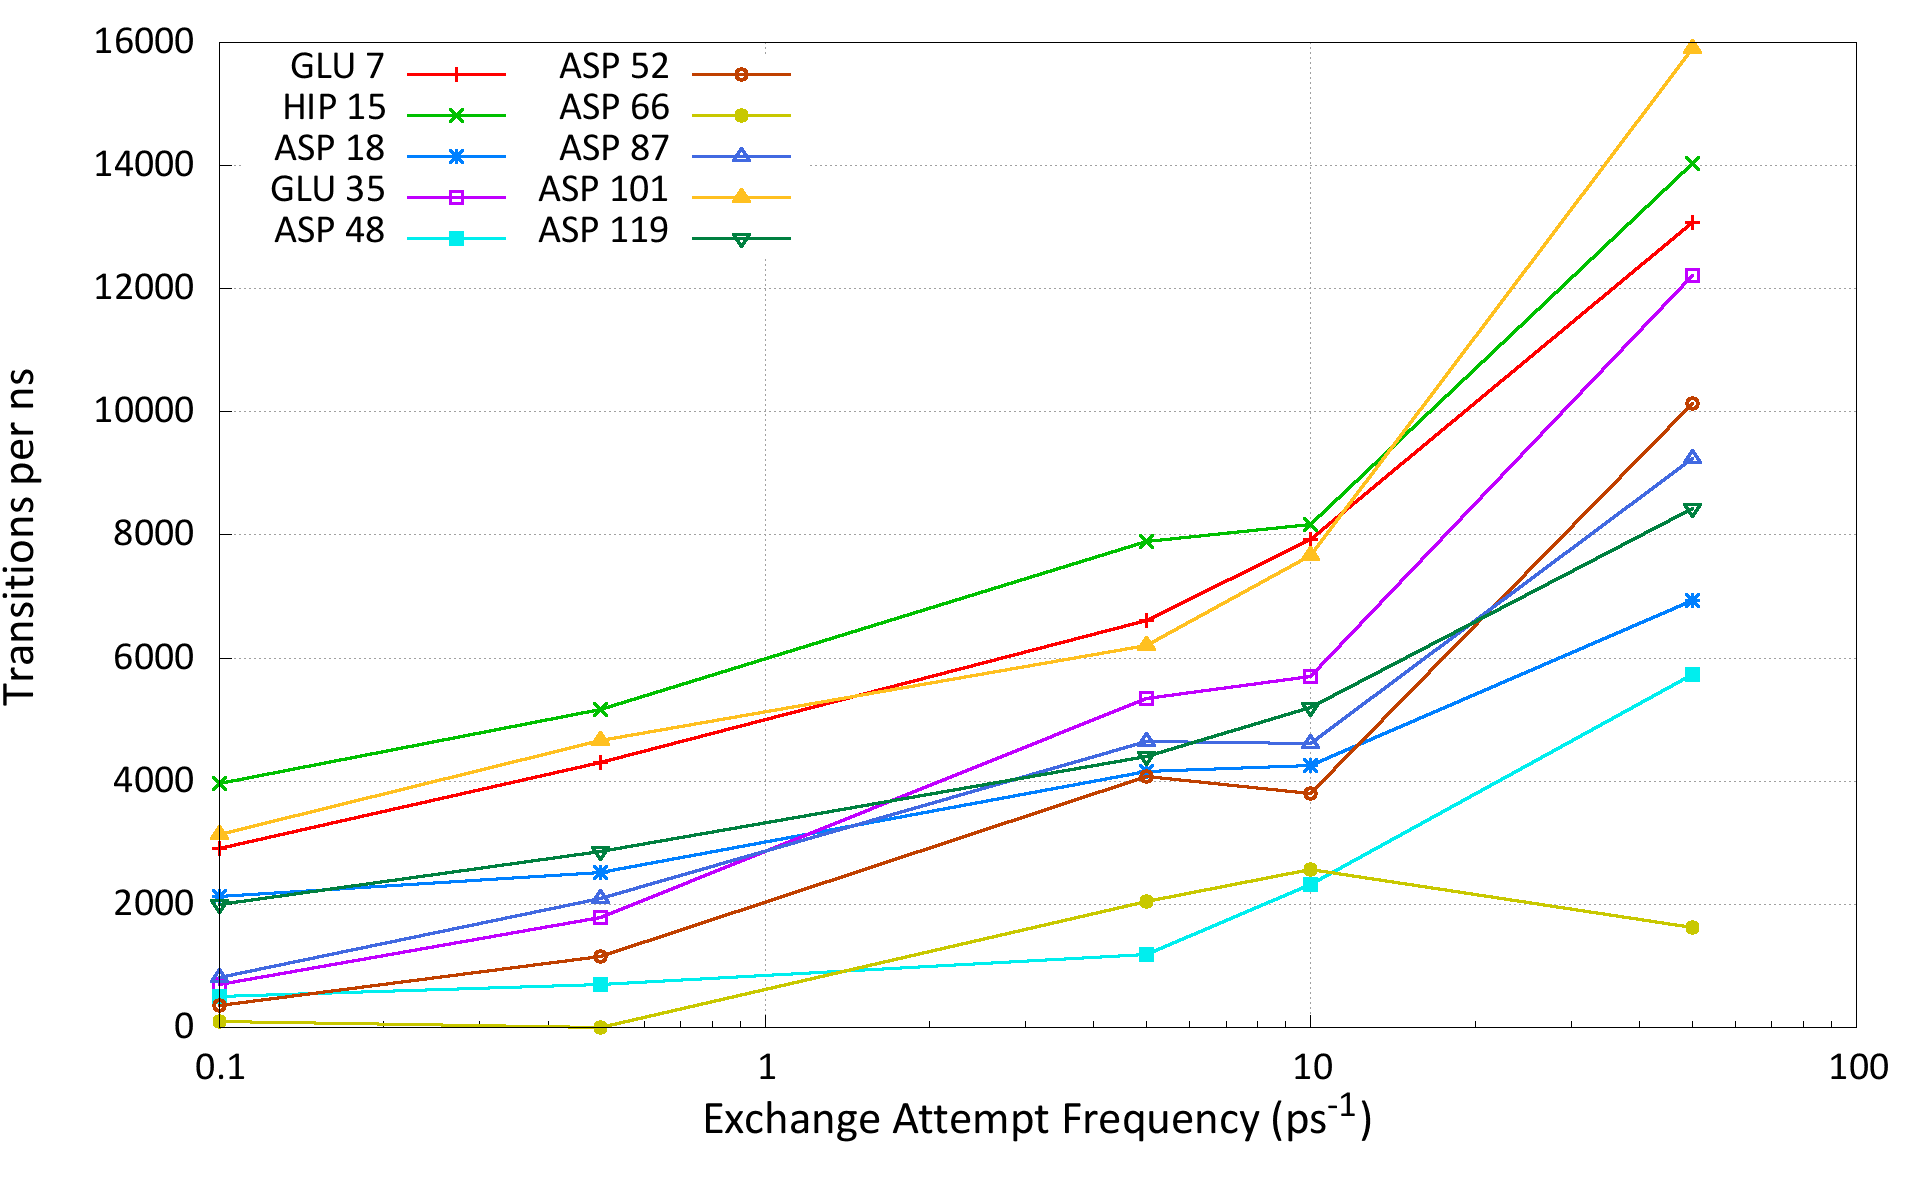
\includegraphics[width=6.5in, height=4.06in]{transitions.png}
 \caption[Number of protonation state transitions per ns of simulation time.]
         {Number of protonation state transitions per ns of simulation time. A
          transition is counted if consecutive snapshots in the ensemble have a
          different number of protons for that residue. The CpHMD results are
          labeled with EAF=0.1 ps\super{-1} to fit on the log-scale.}
 \label{fig3:transitions}
\end{figure}

Simulations that result in more transitions demonstrate enhanced protonation
state sampling, since more protonation state changes occur in the same amount of
time.  All simulations were carried out with the same set of parameters so every
ensemble generated at a given pH will converge to the same result given enough
simulation time.  Therefore, simulations with more transitions will obtain
converged pK\sub{a} values faster.

Fig. \ref{fig3:transitions} shows that increasing EAF dramatically increases the
number of transitions despite the fact that the frequency of attempted
protonation state changes is constant. This is due to the nature of the
probability of accepting a \emph{replica} exchange attempt, which is governed by
Eq. \ref{eq3:ExchSucc}. Because the success of an exchange attempt depends only
on the \emph{net} difference of titrating protons between the two replicas, it
is possible for this net difference to be small, therefore the probability of
accepting the exchange attempt large, even when several residues have different
protonation  states.  Therefore, numerous protonation state changes for
individual residues often accompany a successful exchange of replicas.

\subsection{Enhancing Conformational State Sampling with pH-REMD}

Because conformations and protonation states are coupled, enhanced
conformational sampling from pH-REMD naturally accompanies enhanced protonation
state sampling. In well-designed pH-REMD simulations (\ie pH-REMD simulations
in which efficient mixing occurs in pH-space), each replica contributes
structures to the ensemble at each pH, which serves to increase the number of
conformations visited at each pH.

RMSD is a metric that reflects how different the sampled conformations are from
a reference---in this case the original, minimized crystal structure.  The
histogrammed RMSD data from Fig. \ref{fig3:RMSD} is shown in Fig.
\ref{fig3:RMSD_bin} to allow easier comparison between the different
simulations.

\begin{figure}
 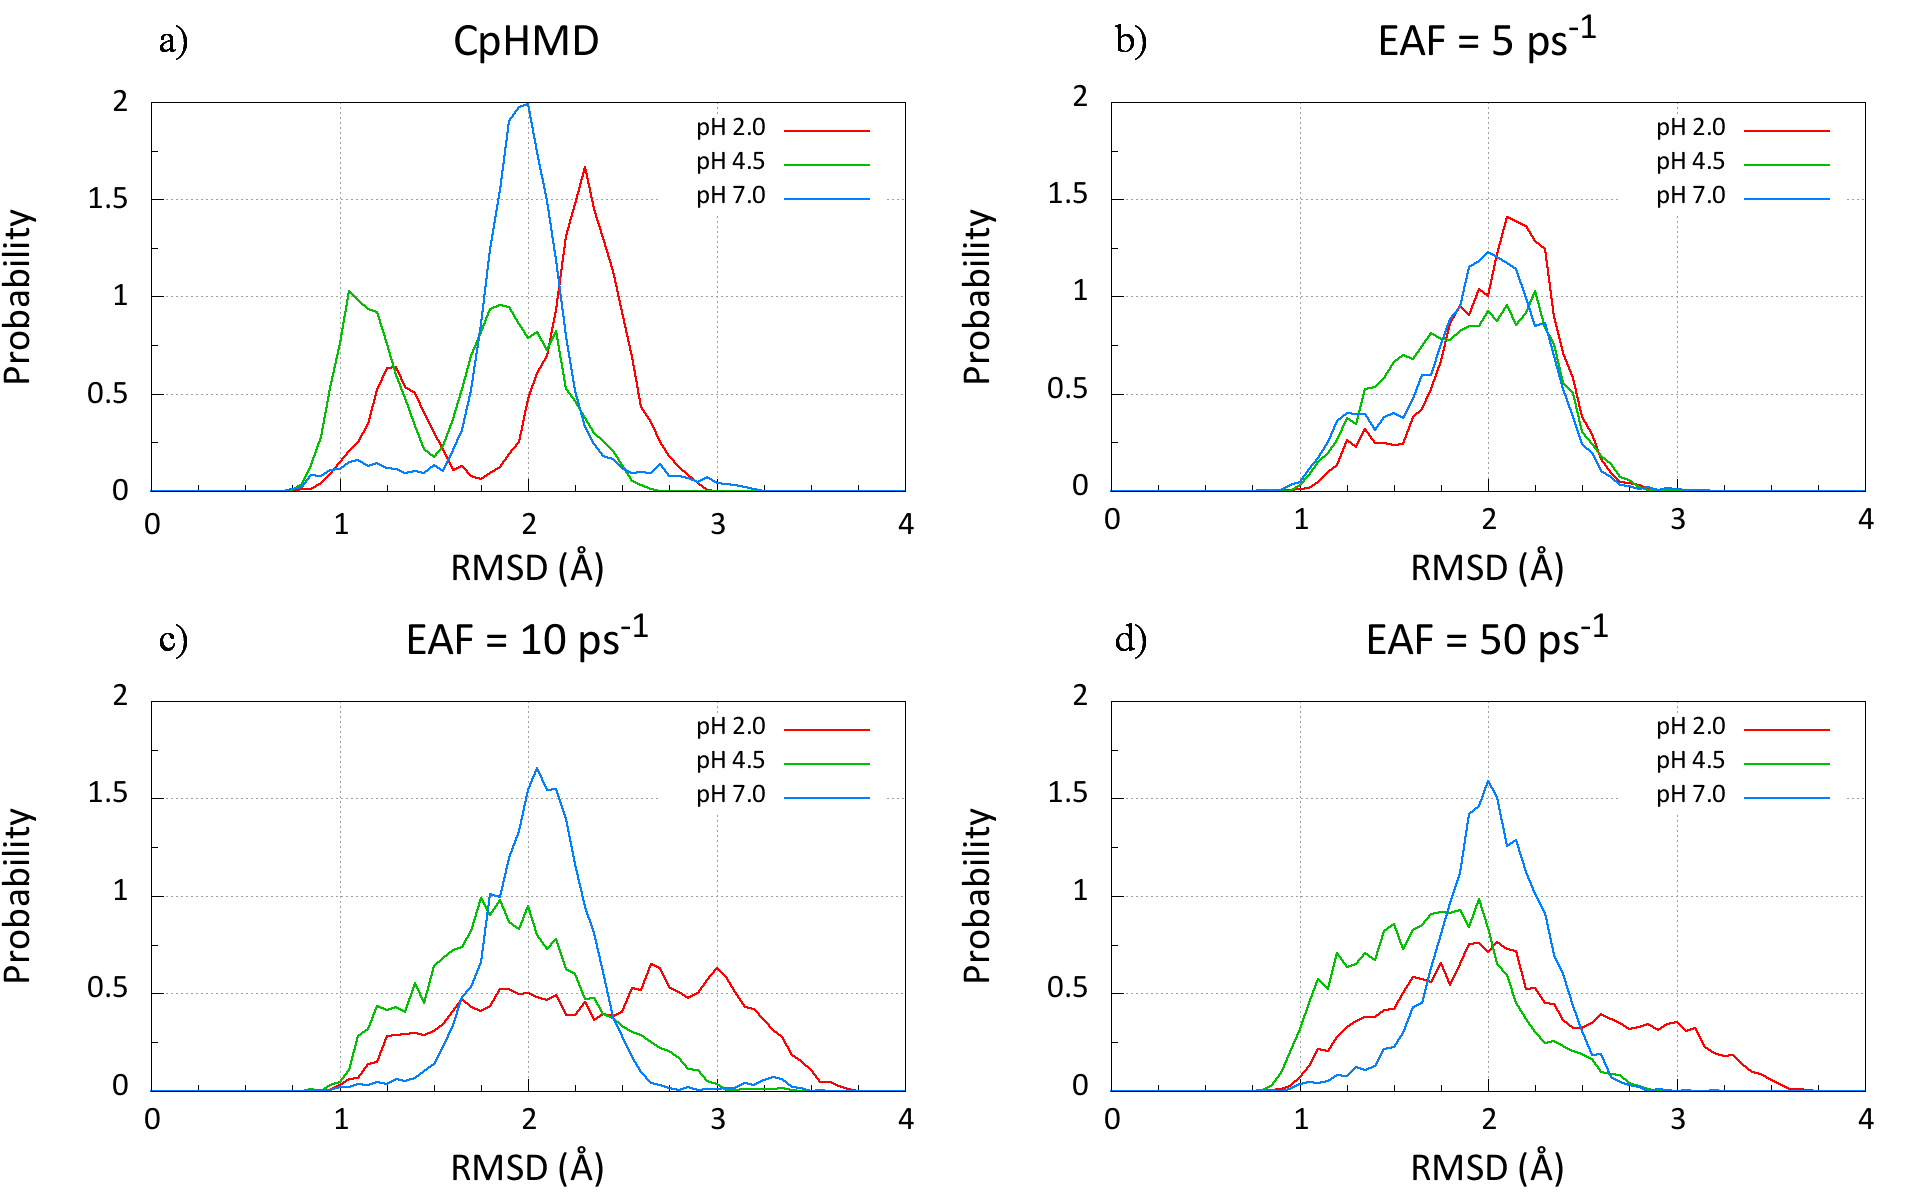
\includegraphics[width=6.5in, height=4.06in]{1AKI_RMSD_Comparison_bins.png}
 \caption{Histogrammed RMSD data for pH 2, pH 4.5, and pH 7 taken from
          simulations run with different EAFs.}
 \label{fig3:RMSD_bin}
\end{figure}

Simulations with higher EAFs traverse the replica ladder more rapidly, allowing
trajectories to break out of local minima that are tied to a particular
protonation state.  The widening bin-widths in Fig. \ref{fig3:RMSD_bin} show
that RMSD-space is explored more thoroughly within the 15 ns timescale sampled
in each simulation as EAF increases to 10 ps\super{-1} (there is no noticeable
difference between the 10 ps\super{-1} and 50 ps\super{-1} EAF).

Because each simulation is subjected to the same set of external constraints
(\eg temperature, pH, solvation model, etc.), each generated ensemble should
represent a subset of the theoretically complete ensemble under these external
constraints.  Because these wider RMSD distribution reflects sampling of more
conformations further from the starting structure, it is almost certain that
these wider distributions at high EAF are thermodynamically `better' (\ie the
ensembles approximate the theoretically complete ensembles better) than their
narrower counterparts in the CpHMD and 5 ps\super{-1} EAF simulations.  The
original RMSD data, plotted in Fig. \ref{fig3:RMSD}, also suggests that pH-REMD
simulations converge more rapidly because those simulations display many
transitions between conformations with different RMSDs.

In addition to sampling more RMSD space than CpHMD simulations, the pH-REMD
simulations also converge to their final RMSD distributions much more rapidly.
To quantify this measure, I used the Kullback-Leibler divergence
\cite{Hamacher2007, McClendon_JChemTheoryComput_2012_v8_p2115} ($D_{KL}$).  The
Kullback-Leibler divergence, calculated via Eq. \ref{eq3:k-l}, quantifies the
similarity between two distinct probability distributions $P(i)$ and $Q(i)$.

\begin{equation}
 D_{KL} = \sum _ {i=1} ^ N P(i) \ln \left( \frac{P(i)} {Q(i)} \right)
 \label{eq3:k-l}
\end{equation}
where $D_{KL}$ is the Kullback-Leibler divergence metric, $i$ is the property of
interest (RMSD in this case), and $P(i)$ and $Q(i)$ are two probability
distribution functions on $i$-space.  For discrete spaces (such as those
obtained by histogramming data), Eq. \ref{eq3:k-l} is represented as a sum (as
shown), but becomes an integral over all of $i$-space for continuous probability
distribution functions $P(i)$ and $Q(i)$.

Fig. \ref{fig3:kullback-leibler} plots $D_{KL}$ calculated from Eq.
\ref{eq3:k-l} where $P(i)$ is the RMSD distribution of each simulation at time
$t$ and $Q(i)$ is the final RMSD distribution of each simulation.  As $P(i)$ and
$Q(i)$ become more similar, $D_{KL}$ tends toward zero.  Therefore, the curves
that approach zero more rapidly approach their final RMSD distribution in a
shorter amount of time.

\begin{figure}
 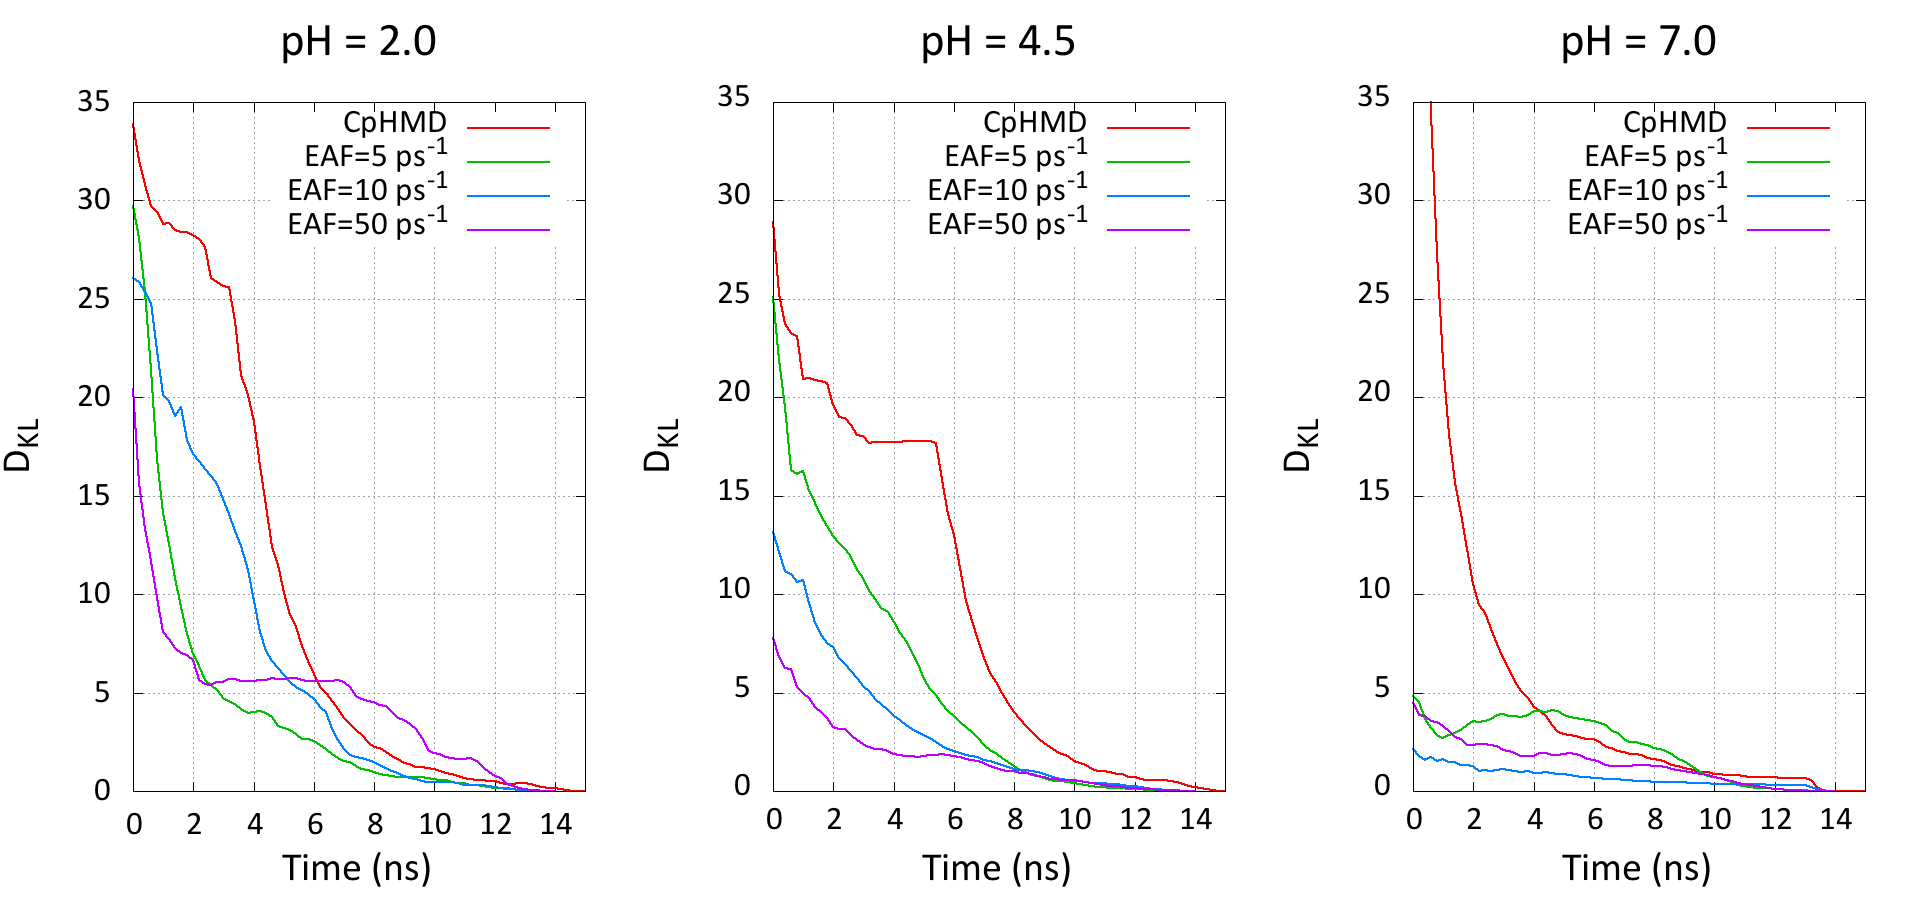
\includegraphics[width=6.5in, height=3.05in]{Kullback_Leibler.png}
 \caption[Kullback-Leibler divergence for each simulation calculated via Eq.
          \ref{eq3:k-l}.]
         {Kullback-Leibler divergence for each simulation calculated via Eq.
          \ref{eq3:k-l}.  $P(i)$ is the RMSD histogram of the indicated
          simulation at time $t$ and $Q(i)$ is the RMSD histogram of the entire
          indicated simulation.  Values closer to zero indicate distributions of
          higher similarity.}
 \label{fig3:kullback-leibler}
\end{figure}

The pH-REMD simulations not only explore more RMSD space than the corresponding
CpHMD simulations, but they characterize this larger space more rapidly as well,
since they converge to their final distribution faster than CpHMD.  Furthermore,
the simulations with an EAF of 10 ps\super{-1} and 50 ps\super{-1} typically
converge faster than the one with an EAF of 5 ps\super{-1}.  The only exception
in this case, including the pHs not shown in Fig. \ref{fig3:kullback-leibler},
is the simulation at pH 2.  In general, simulations with EAF 10 ps\super{-1} and
50 ps\super{-1} are indistinguishable with respect to RMSD.

At pH 2, the RMSD distribution of the EAF=5 ps\super{-1} simulation is much
narrower than the corresponding distributions at EAF 10 ps\super{-1} and 50
ps\super{-1}.  Therefore, it's not surprising that the $D_{KL}$ of the 5
ps\super{-1} EAF simulation converges more rapidly than the higher EAFs.  In
general, however, pH-REMD simulations with high EAFs sample more RMSD space more
efficiently than CpHMD and simulations with low EAFs.

To probe the nature of the conformational flexibility of HEWL at different EAFs,
I calculated the average atomic fluctuations for each residue from the average
structure. These fluctuations provide insight into the flexible regions of the
protein, giving a more fine-grained, structural analysis than RMSD does.  The
results, shown in Fig. \ref{fig3:fluxes}, show that the same parts of HEWL are
generally flexible for each simulation, but the pH-REMD simulations tend to
display enhanced flexibility compared to the CpHMD simulations.  Again, because
each simulation samples from the same ensemble subject to the same thermodynamic
constraints, this increased flexibility suggests that the simulations at high
EAF converge to the true ensemble more rapidly than the CpHMD simulations and
the pH-REMD simulations with a low EAF.

\begin{figure}
 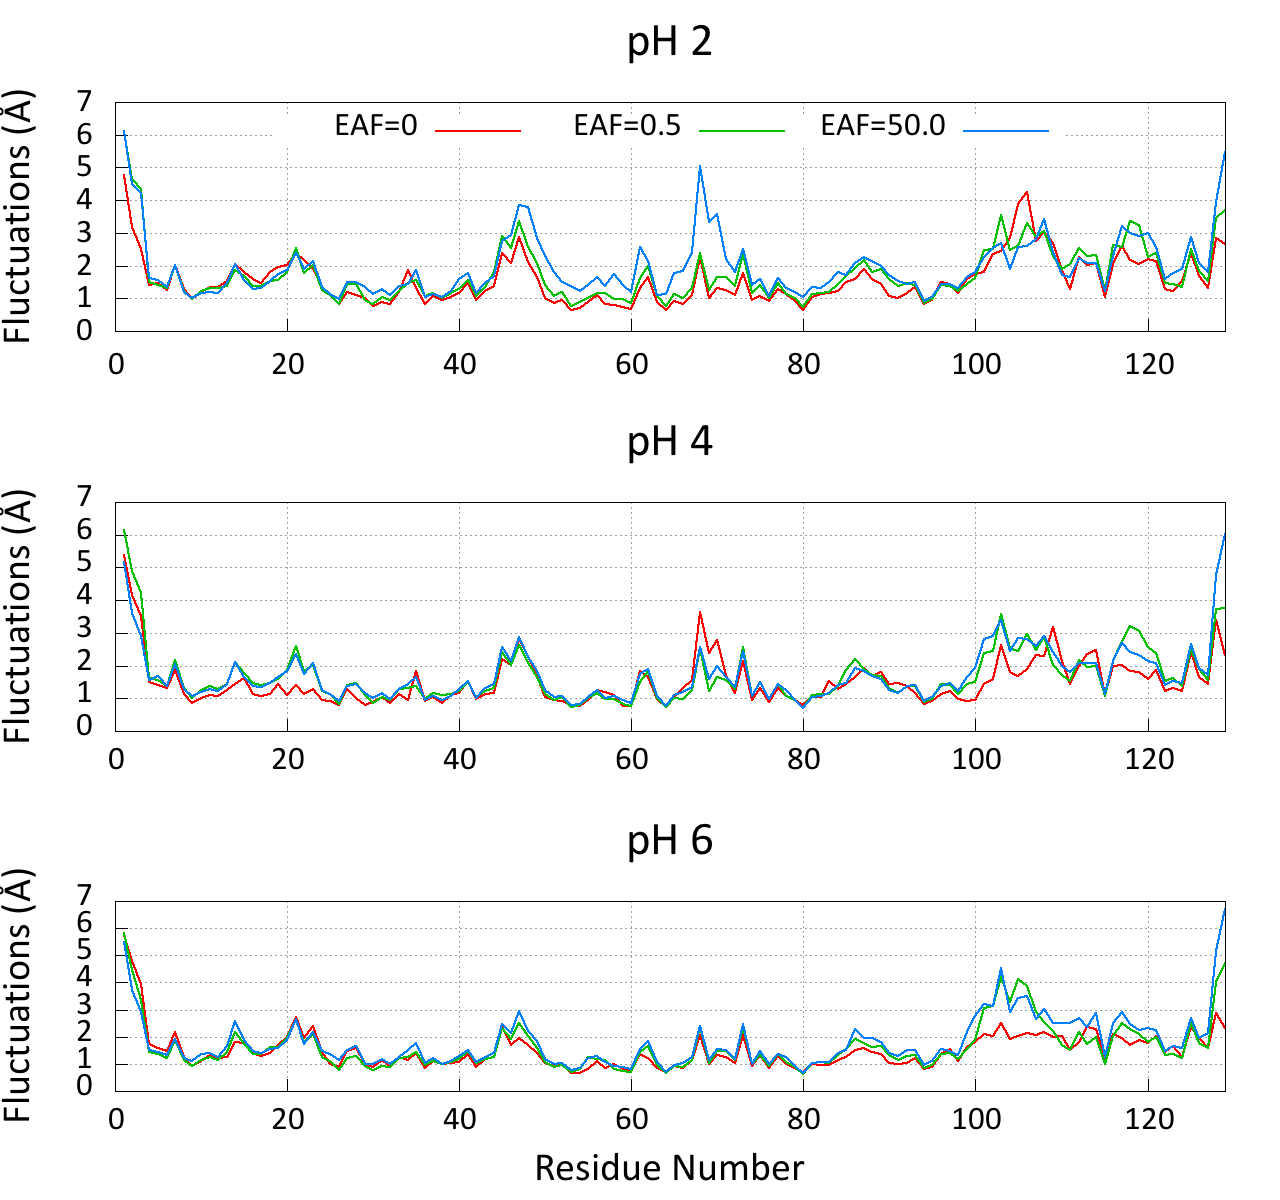
\includegraphics[width=6.5in, height=6.09in]{residue_fluctuations.png}
 \caption[Average atomic fluctuations for each residue relative to the average
          structure of the ensemble.]
         {Average atomic fluctuations for each residue relative to the average
          structure of the ensemble. Data are shown for CpHMD, low EAF (0.5
          ps\super{-1}) and high EAF (50 ps\super{-1}).}
 \label{fig3:fluxes}
\end{figure}

While the overall flexibility in pH-REMD simulations is increased with respect
to the CpHMD simulations, the dynamics still reveal different behavior at
different pH.  In particular, the region between residues 100 and 120 shows
drastically increased flexibility at pH values higher than 4 for the pH-REMD
compared to the CpHMD simulations.

Furthermore, the region around residue 70, which shows heightened flexibility at
pH 2 (Fig. \ref{fig3:fluxes}), contains the problematic titratable residue Asp
66.  This increased flexibility at high EAF is the likely explanation why Asp 66
protonates at low pH in the pH-REMD simulations but not in the CpHMD simulation
where this loop is substantially less flexible.

To probe the pH-dependence of HEWL dynamics further, I plot the distributions
of the distance between the carboxylate carbons of the catalytic residues Asp 52
and Glu 35 at each pH.  Because Asp 52 and GLU 35 are the catalytic residues in
HEWL, this behavior may have important implications in the HEWL catalytic
activity profile as a function of pH.

Fig. \ref{fig3:cat_dist} shows that only the simulation run at pH 5 samples
conformations in which Asp 52 and Glu 35 are closely interacting for the CpHMD
simulations.  Furthermore, the simulation at pH 5 spends roughly 75\% of its
time `stuck' in this close interaction.  It is highly unlikely that this
interaction is so strong at pH 5, yet is almost non-existent at pH 4.5 and 5.5.
More likely, Fig. \ref{fig3:cat_dist} suggests that the CpHMD simulation run at
pH 5 became trapped while trajectories at other pH values were unable to enter
this conformational bin within the 16 ns of simulation.

\begin{figure}
 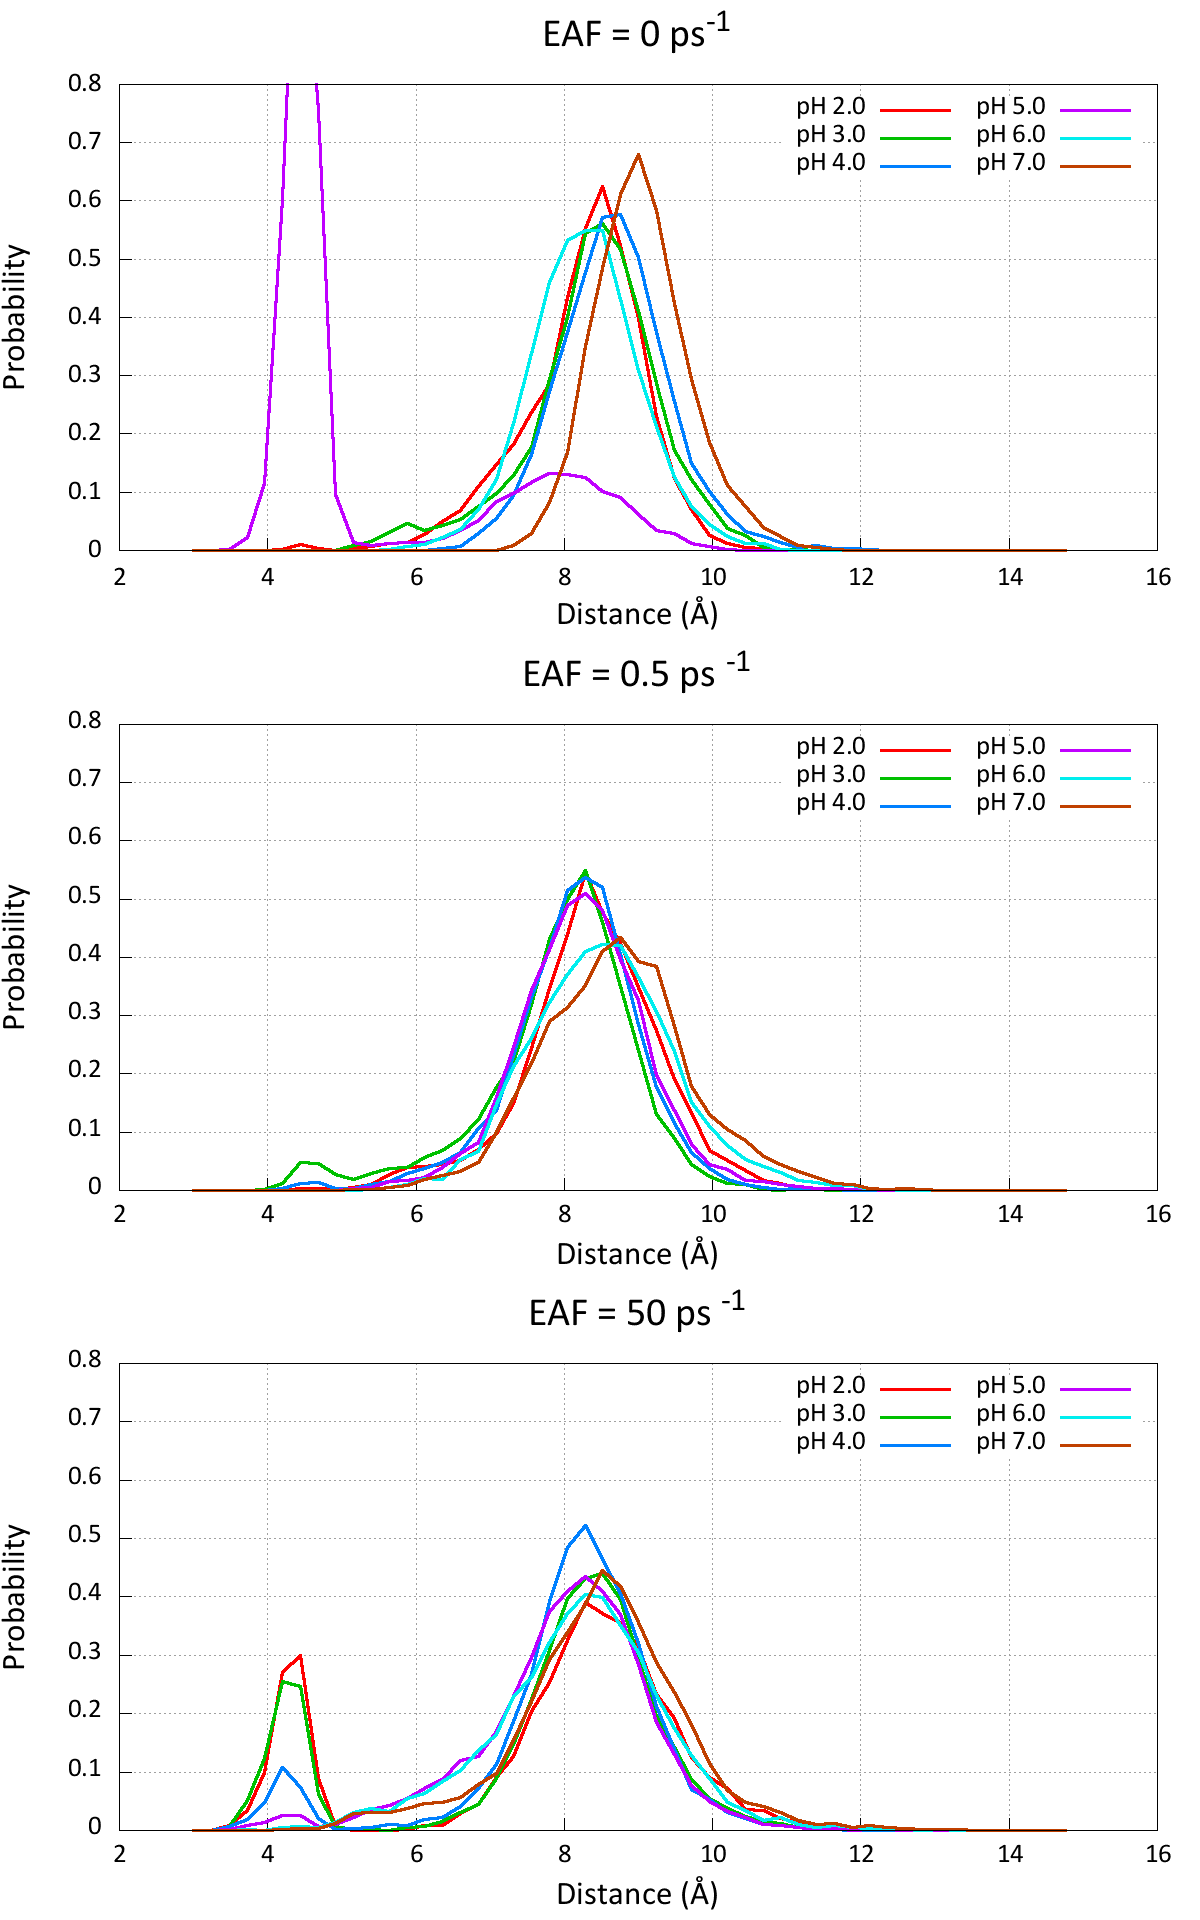
\includegraphics[width=4.06in, height=6.5in]{Catalytic_Distances.png}
 \caption{Distributions of the Asp52-C$^\gamma$--Glu35-C$^\delta$ carboxylate
          carbons. Asp 52 and Glu 35 are the catalytic residues of HEWL.}
 \label{fig3:cat_dist}
\end{figure}

pH-REMD simulations with a high EAF easily overcome this barrier within the
simulation time scale.  The distributions from pH-REMD simulations with a 50
ps\super{-1} EAF display more expected behavior, given that the calculated
pK\sub{a}s of Asp 52 and Glu 35 are 2.30 and 4.98, respectively
(Table \ref{tbl3:pkas}).  This interaction is likely strongest when one of the
carboxylates is protonated and the other is deprotonated, and it is likely
weakest when both are deprotonated.  Therefore, this interaction should be
strongest at a pH between 2.30 and 4.98.

The Asp 52---Glu 35 interaction is the strongest at pH 2.5 and decays as the pH
either increases or decreases.  At pH 2.5, Asp 52 is most likely deprotonated
while Glu 35 is most likely protonated.  At pH 2.0, both residues are likely to
be protonated, resulting in a slightly weaker interaction.  However, this is
still more favorable than when both residues are deprotonated, so the
interaction becomes significantly weaker as the pH increases.

Furthermore, tight coupling between Asp 52 and Glu 35 likely induces non-HH
behavior as these residues no longer titrate independently.  This explains why
the Hill coefficient for Asp 52, reported in Table \ref{tbl3:pkas}, is more
significantly shifted away from 1---to 0.75---for the EAF of 50 ps\super{-1}.
Over the pH range that contains the Asp 52 inflection point, Fig.
\ref{fig3:cat_dist} shows that the interaction between the two active site
residues is strong.  Over the pH range that contains the Glu 35 inflection
point, however, the interaction is weak, causing the Glu 35 titration to display
nearly ideal Henderson-Hasselbalch behavior.

To better illustrate the pH-dependence of the Glu 35 -- Asp 52 interaction
depicted in Fig. \ref{fig3:cat_dist}, (at 50 ps\super{-1} EAF) I integrated
each of the distributions from 0 \mbox{\normalfont \AA} to 5 \mbox{\normalfont
\AA} and plotted the result against pH, shown in Fig. \ref{fig3:cat_dist_int}.

\begin{figure}
 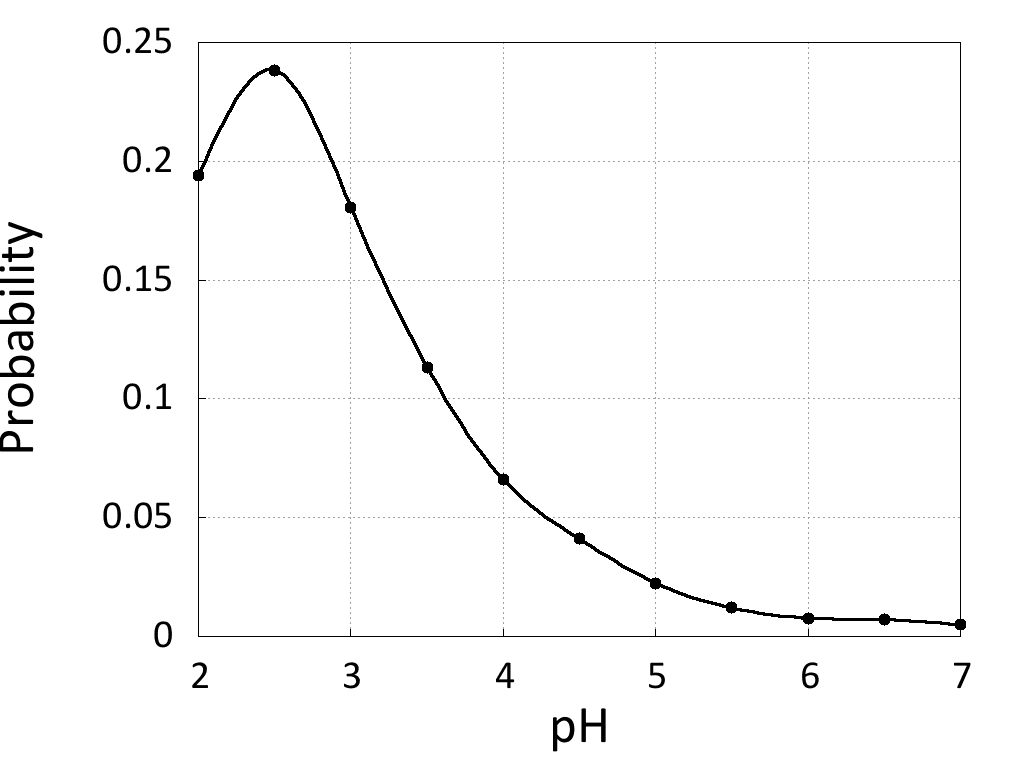
\includegraphics[width=6in, height=4.5in]{Catalytic_Distances_Int.png}
 \caption{Fraction of simulation with the Glu 35 -- Asp 52 distance shorter than
          5 \mbox{\normalfont \AA} vs. pH.}
 \label{fig3:cat_dist_int}
\end{figure}

\subsection{Scalability With Increasing Exchange Attempt Frequency}

It is important when selecting a simulation protocol to consider the performance
implications of each of the choices, since there is often a trade-off between
computational expense and theoretical rigor.  As
\citeauthor{Mongan_JComputChem_2004_v25_p2038} demonstrated in their work, the
CpHMD method implemented in Amber is only marginally more expensive than
traditional MD with constant protonation states.
\cite{Mongan_JComputChem_2004_v25_p2038}  Here, I will discuss the performance
implications of increasing the EAF of pH-REMD simulations.

The computational cost of the pH-REMD simulations is the sum of the cost of the
underlying CpHMD method \cite{Mongan_JComputChem_2004_v25_p2038} and the cost of
the replica exchange attempts.  The exchange success probability in pH-REMD
simulations is governed by Eq. \ref{eq3:ExchSucc} and can be implemented so that
the computational cost of each exchange attempt is negligible.  The replicas of
every simulation were carried out on 24 processors on NICS Keeneland
\cite{Vetter2011} so the simulation efficiency, measured in terms of ns of
simulation per day, can be directly compared. The average results obtained for
each EAF is summarized in Table \ref{tbl3:timings}.

\begin{table}
 \caption[Average timings for CpHMD and pH-REMD simulations.]
         {Average timings for CpHMD and pH-REMD simulations. CpHMD simulations
          used 24 processors, whereas pH-REMD simulations used 288
          processors---24 per replica. All simulations were performed on NICS
          Keeneland. \cite{Vetter2011}}
 \begin{tabular}{rc}
  \hline
  EAF (ps \super{-1}) & Efficiency (ns/day) \\
  \hline
  0.0 & 7.56 \\
  0.5 & 6.81 \\
  5.0 & 6.55 \\
  10.0 & 6.72 \\
  50.0 & 6.70 \\
  \hline
 \end{tabular}
 \label{tbl3:timings}
\end{table}

The decreased performance from the CpHMD simulation (EAF=0.0 in
Table \ref{tbl3:timings}) to the EAF=5.0 ps\super{-1} simulations arises from
the fact that REMD simulations in Amber currently require each replica to
perform the same number of MD steps between exchange attempts.  This
synchronization causes each replica to run only as fast as the slowest replica.

The pH-REMD simulations are run with 288 processors (12 replicas with 24
processors each), whereas the CpHMD simulations are run each replica
independently---with only 24 processors.  Therefore, the synchronization of the
replicas in REMD is responsible for the 10\% performance reduction between the
CpHMD simulation and the pH-REMD simulation with an EAF of 0.5 ps\super{-1}
(attempting exchanges every 1000 integration steps).

Increasing the EAF of pH-REMD simulations from 0.5 ps\super{-1} to 50.0
ps\super{-1} (attempting exchanges every 10 steps) results in a 1\% reduction in
average simulation efficiency---a value that falls well within the fluctuations
between two different simulations with the same EAF run on the same machine.
Given the lack of performance degradation as EAF increases and the improved
performance of simulations as EAF increases, the best EAF to use with the
presented pH-REMD implementation is one where exchanges are attempted every 10
to 50 integration steps (10.0 ps\super{-1} and 50.0 ps\super{-1} in this study,
respectively).

\section{Conclusion}

In this study, I have shown that pH-REMD effectively enhances sampling from the
semi-grand canonical ensemble compared to CpHMD in the case of hen egg-white
lysozyme.  The titration curves generated from pH-REMD simulations are
considerably less noisy than the analogous titration curves generated from CpHMD
simulations, and they fit to the Hill equation much better.  Furthermore,
pK\sub{a}s calculated from pH-REMD simulations converge faster and achieve
better precision than CpHMD.

In some cases, pH-REMD can effectively cross potential energy barriers that trap
residues in CpHMD simulations.  In the case of the Asp 66 residue in HEWL, CpHMD
simulations were unable to obtain noticeable protonation fractions even at a pH
as low as 2 when started from the 1AKI crystal structure.  Utilizing pH-REMD
simulations with a rapid EAF, I obtained a titration curve with a Hill
coefficient close to 1 and a calculated pK\sub{a} that compares well to
experiment.

I have demonstrated that increasing the EAF improves sampling and convergence
of several observables in this study.  Asp 66 titrates more efficiently with a
high EAF due to enhanced the mobility of flexible regions of the protein.
Furthermore, analysis of the distance between the catalytic residues Asp 52 and
Glu 35 show that increasing the EAF can provide valuable chemical insight into
biologically significant pH-dependent behavior of proteins.  Similarly to past
work with temperature REMD, \cite{Sindhikara2008,Sindhikara2010} high EAFs give
rise to more rapid convergence.

Replica exchange methodologies can be implemented efficiently to reduce the cost
of each exchange attempt.  In pH-REMD, the exchange success probability,
governed by Eq. \ref{eq3:ExchSucc}, involves only trivial mathematics so the
cost of evaluating Eq. \ref{eq3:ExchSucc} is negligible.  For efficient REMD
implementations, like the one presented in this work, I recommend setting the
EAF to at least 10 ps\super{-1}, although some improvement is still seen with
higher EAFs.

\citeauthor{Chodera_JChemPhys_2011_v135_p194110}
\cite{Chodera_JChemPhys_2011_v135_p194110} provide an explanation for the
improved efficiency of high EAFs by relating it to Gibbs' sampling and the
effect high EAF has on `state space' sampling (pH-space in this study).  In
their paper, \citeauthor{Chodera_JChemPhys_2011_v135_p194110} propose
enhancements to the exchange process in REMD simulations, such as exchanges
between non-adjacent neighbors in `state space' as well as attempting multiple
exchanges before resuming dynamics. \cite{Chodera_JChemPhys_2011_v135_p194110}

pH-REMD is likely to benefit by attempting exchanges between non-adjacent
neighbors, since the difference in pH between replicas is small.  Given the
simplicity of the exchange probability equation (Eq. \ref{eq3:ExchSucc}), the
exchange success rate can be calculated between any two replicas over the course
of the pH-REMD simulation.  The calculated success rates show a non-negligible
probability of accepting exchange attempts between replicas up to 2 pH units
away from each other (\ie separated by 3 replicas).
